\documentclass[a4paper, 11pt, twoside]{report}
% add the packages
\usepackage{graphicx}
\usepackage{bm}
\usepackage{pdfpages}
\usepackage{amsmath}
\usepackage{amssymb}
\usepackage[ruled,vlined]{algorithm2e}
\usepackage{algpseudocode}
\usepackage{fixltx2e}
\usepackage[explicit]{titlesec}
\usepackage{float}
\usepackage[nottoc]{tocbibind}
\usepackage[english]{babel} 
\usepackage[da,english]{stthesis}
\usepackage{caption}
\usepackage{comment}
\usepackage{subcaption}
\usepackage{geometry}
\usepackage{url}
\usepackage[intoc]{nomencl}
\usepackage{color,soul}
\usepackage{tikz}
\usepackage[justification=centering]{caption}
\newcommand*\circled[1]{\tikz[baseline=(char.base)]{
            \node[shape=circle,draw,inner sep=1.5pt] (char) {#1};}}
            
\geometry{a4paper, top=40mm, left=45mm, right=35mm, bottom=40mm, headsep=10mm, footskip=12mm}


\let\oldemptyset\emptyset
\let\emptyset\varnothing

\graphicspath{{pics/}}

\setcounter{secnumdepth}{3}
\setcounter{tocdepth}{3}

\captionsetup{font=sf}
\makenomenclature
\setlength\nomlabelwidth{2.5cm}
\begin{document}

\pagenumbering{gobble}
\thispagestyle{empty}

\begin{flushleft}
	
\includegraphics[height=1.65cm]{tu.pdf}
\end{flushleft}

\parindent0pt
\rule{140mm}{0.3mm}
\newline
\textbf{Faculty of Computer Science}\\ Distributed System Engineering, Chair for System Engineering
\newline
\rule[2.5mm]{140mm}{0.3mm}

\begin{center}
	\vspace{2cm}
	\Large
	\textsc{Master Thesis}\\
	
	\vspace{1cm}
	\LARGE
	\textbf{Quality-Driven Disorder Handling for Sliding-Window Joins}\\
	\vspace{2cm}
	\Large
	Jun Sun\\
\end{center}

\begin{flushleft}
	\vspace{4cm}
	\begin{tabular}{ll}
	Professor:  & Prof. Dr.  Christof Fetzer\\
	Supervisor: & M.Sc. Yuanzhen Ji (SAP SE) \\
	\\
	\multicolumn{2}{l}{Submitted on  June 9th, 2015} \\
	\end{tabular}
\end{flushleft}
\cleardoublepage

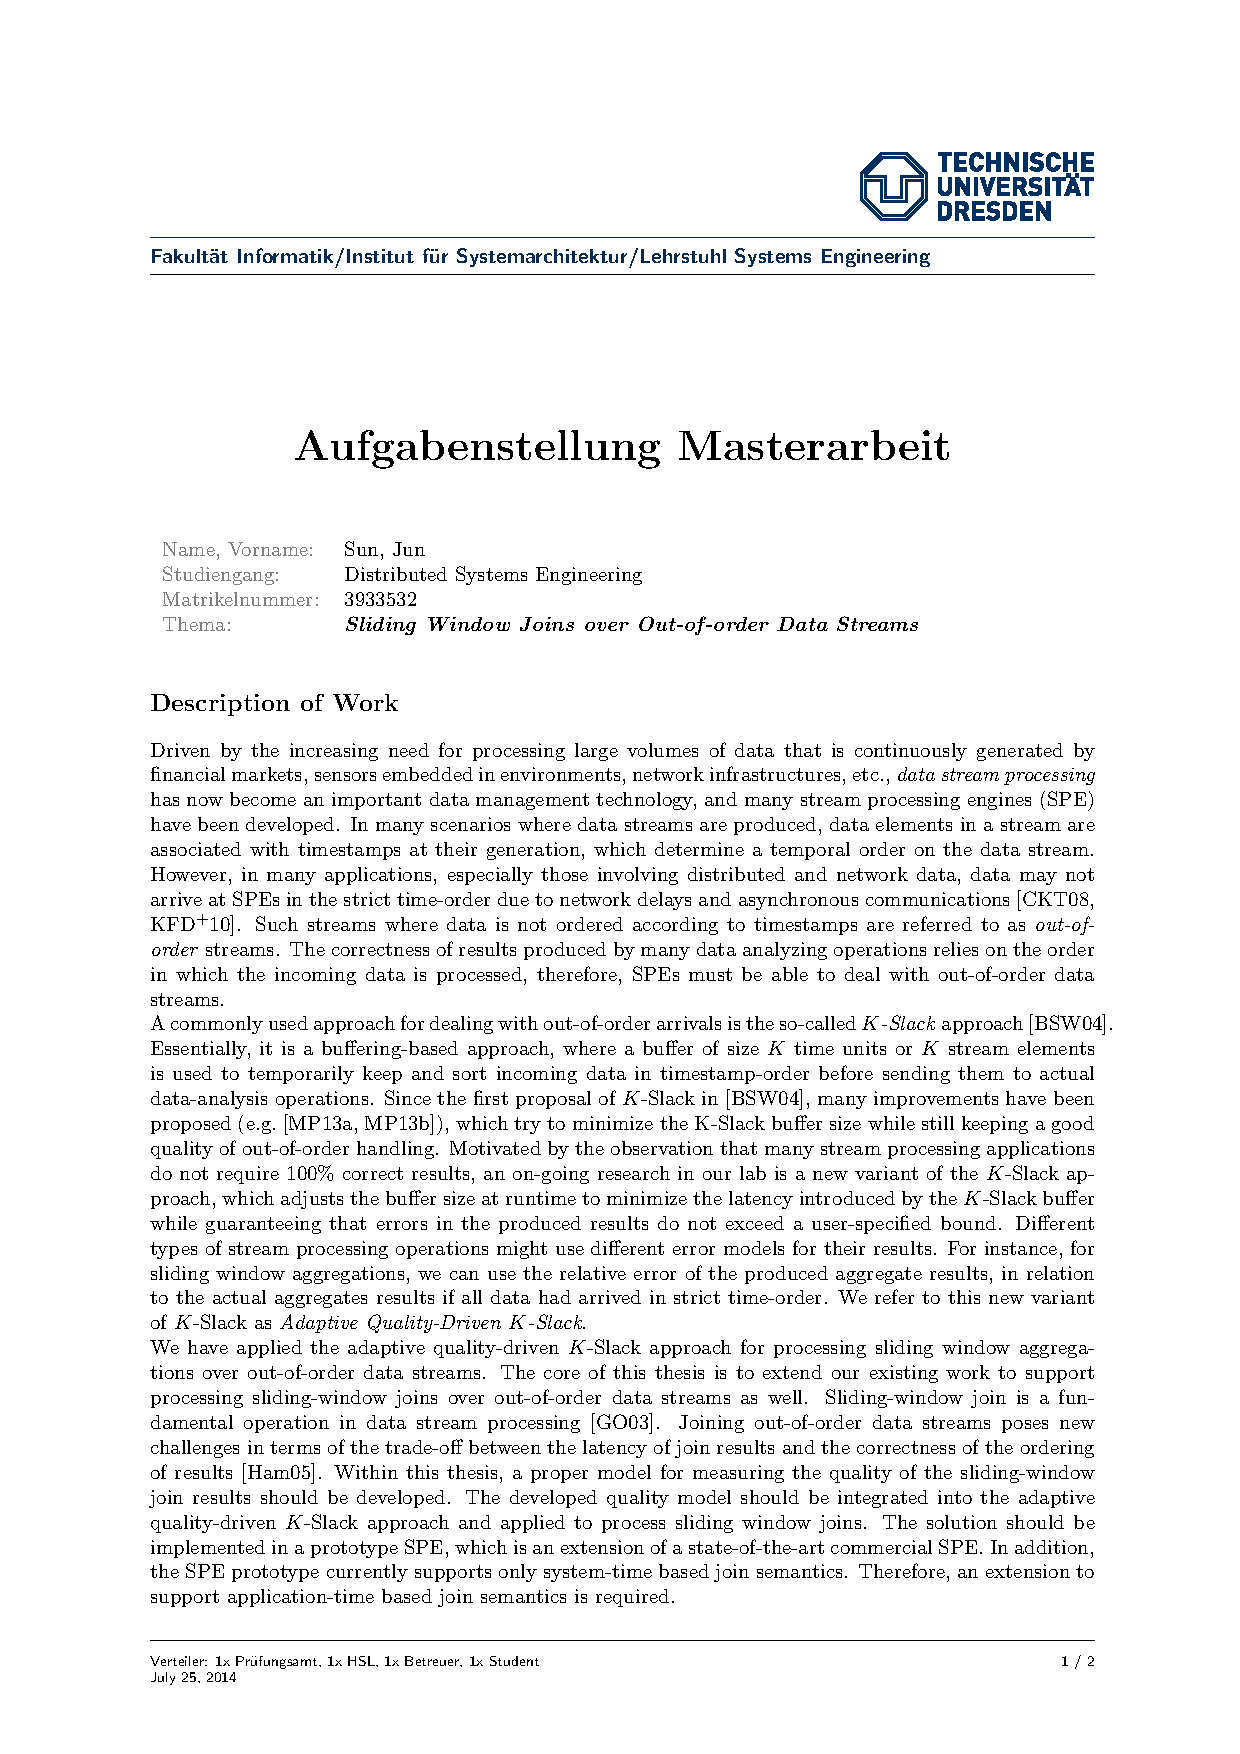
\includepdf[pages={-}]{ThesisDescription.pdf}
\cleardoublepage


\includepdf[pages={-}]{ThesisApplication.pdf}
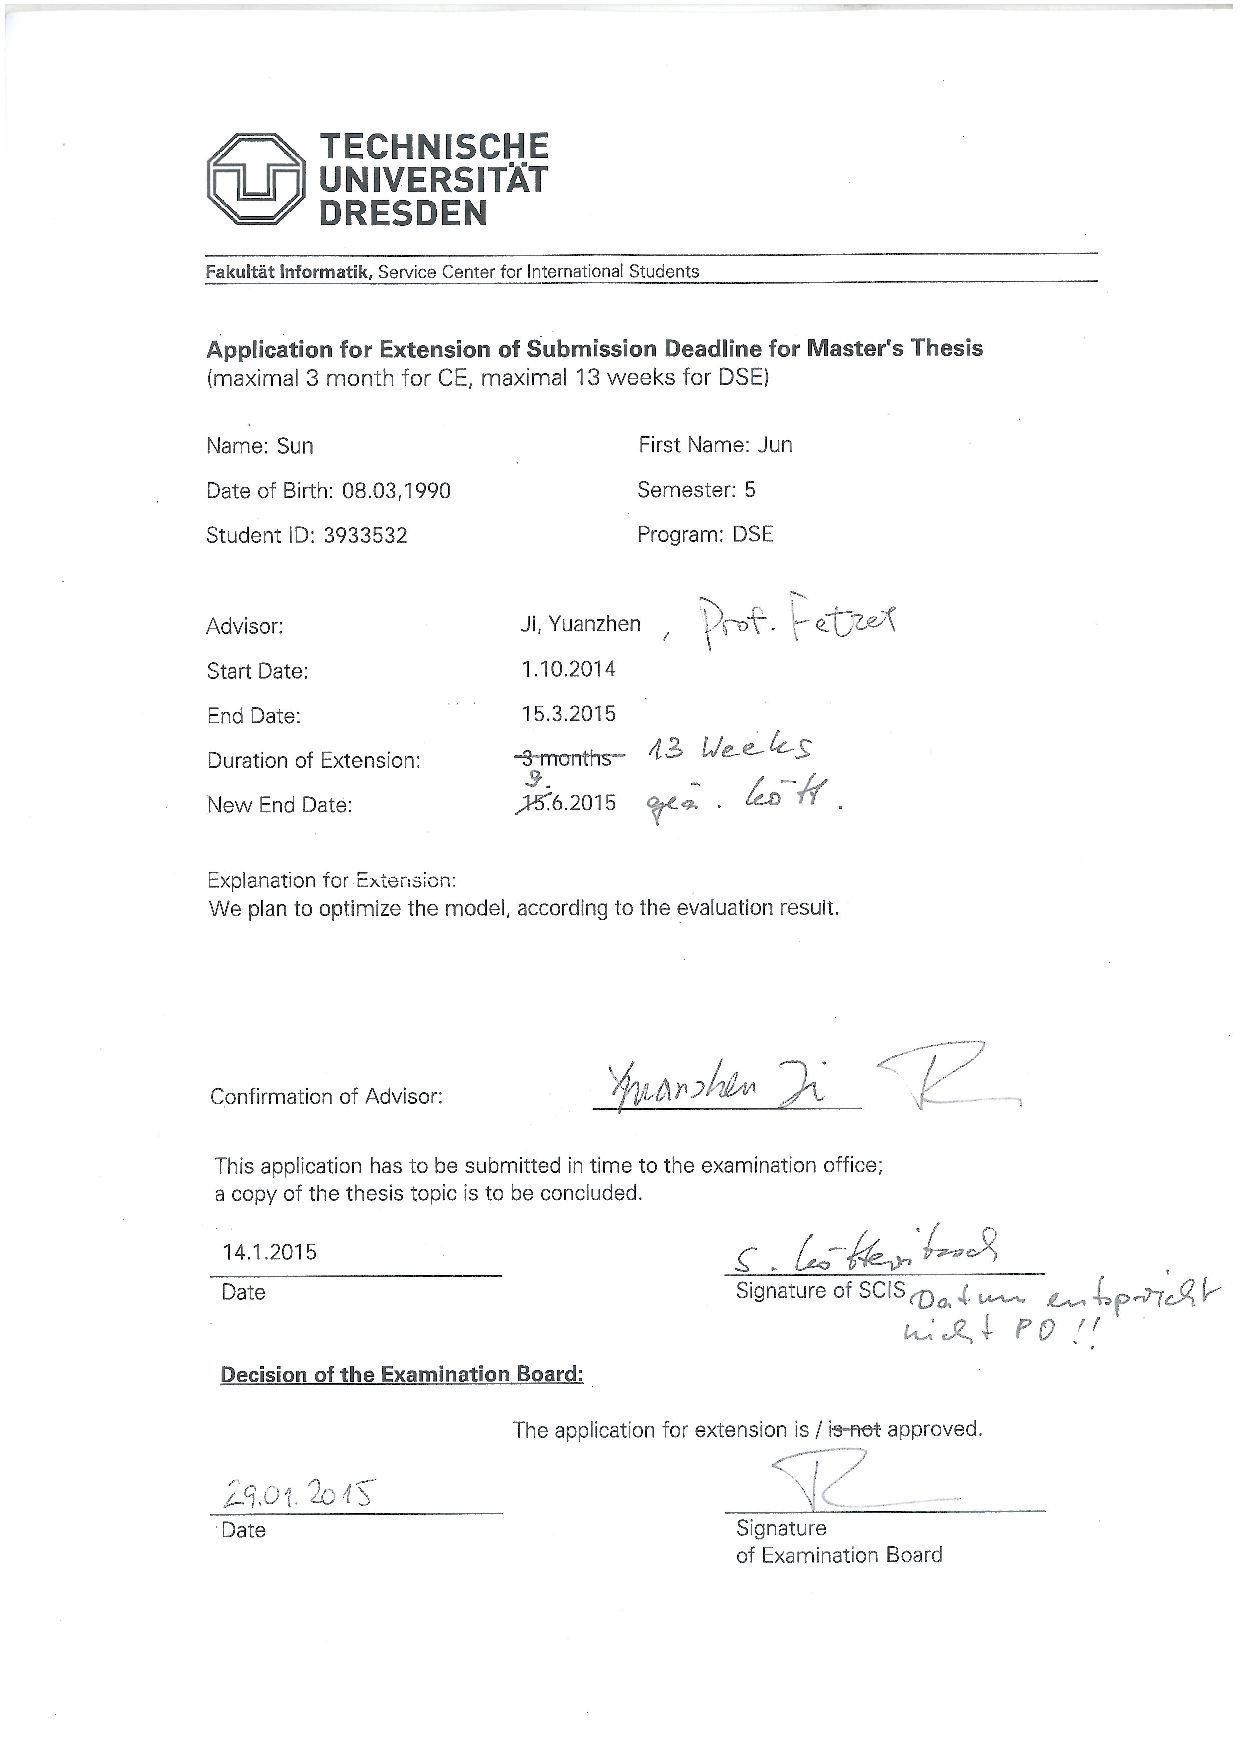
\includepdf[pages={-}]{Extension.pdf}
\cleardoublepage

\begin{abstract}

In data stream processing systems, stream processing engines (SPE) can perform various types of operations, e.g., AGGREGATE, UNION, JOIN, over incoming data streams. When the arrival order of the data is the same as the order of their generation, the SPE can produce results with no extra effort. However, it is often possible that the arrival order cannot be guaranteed due to uncontrollable factors such like network delay, thus the SPE is no longer able to keep the result semantic of the origin without exploiting disorder handling approaches, e.g., a buffer to wait for late arriving data, which causes result latency.\\

In this paper, we concentrate on the operation of sliding-window JOIN. In order to minimize the result latency while giving a high-quality result satisfying users' demands, we use the state-of-the-art quality metric for data stream JOIN operation, and propose a probabilistic model based on the observation of late arrival patterns that the incoming data streams exhibit. We apply this model to the SPE, in order to do online trade-off between result latency and result quality, i.e., to adjust the buffer size on the fly.\\

We implement our proposal in SAP Sybase Event Stream Processor (ESP). Experimental evaluations with real-world out-of-order data streams validate the effectiveness of our approach, which causes only modest computational overhead for result quality monitoring and buffer size adaptation.

\end{abstract}
\cleardoublepage

\tableofcontents
\cleardoublepage

\pagenumbering{arabic}

\chapter{Introduction}

Nowadays, data stream processing systems are widely used in different areas like sports, finance, fraud detection and so on \cite{Mutschler:2013:RSP:2488222.2488263}. According to the \textit{continuous queries} \cite{babu2001continuous} the users define, stream processing engines (SPE) can perform a variety of operations, e.g., AGGREGATE, UNION, JOIN over unbounded data streams and produce result streams. Among these operations, \textit{sliding-window} JOIN is an ordinary but important one, which is used in many stream processing applications. The following example gives a typical sliding-window JOIN query with two input streams.

\begin{verbatim}
SELECT 
  MAX(S.Timestamp, T.Timestamp) as Timestamp, S.ItemID as ItemID,
  S.Name, T.Order
FROM SensorOne as S KEEP 3 SECOND, SensorTwo as T KEEP 2 SECOND
SLIDE 1 SECOND
WHERE S.ItemID = T.ItemID
\end{verbatim}

In the query given above, two data sources generate data as $tuples$ associated with timestamps. For example, \texttt{SensorOne} generates tuples as \texttt{(Timestamp, ItemID, Name)}, and \texttt{SensorTwo} generates tuples as \texttt{(Timestamp, ItemID, Order)}. The SPE then joins the two input data streams containing continuous tuples from the two data sources respectively. The \texttt{KEEP} clauses define the sliding window sizes over two input streams. \texttt{SLIDE 1 SECOND} means that both windows slide every 1 second. The \texttt{WHERE} clause defines the join condition. The timestamp of a result tuple is defined as the maximum of the two timestamps of the two component input tuples\footnote{There are different strategies regarding the timestamps of the result tuples. In this thesis we use the greater timestamp of two element tuples as the timestamp of the result tuple, as in \cite{ayad2004static}.}.\\

Executing this query over the data streams S and T shown in Figure \ref{fig:intro-example} we will get an output stream R. At global time 2, tuple (1, 0199, Alice) from Stream S joins tuple (2, 0199, Burger) from Stream T; and tuple (2, 0200, Bob) from Stream S joins tuple (1, 0200, Coke) from Stream T. At global time 4, tuple (3, 0201, Carol) from Stream S joins with tuple (4, 0201, Burger) from Stream T. Note that tuple (5, 0200, Dave) from Stream S does not join with tuple (1, 0200, Coke) from Stream T, because they are not in window at the same time.\\

\begin{figure}[h]
\centering
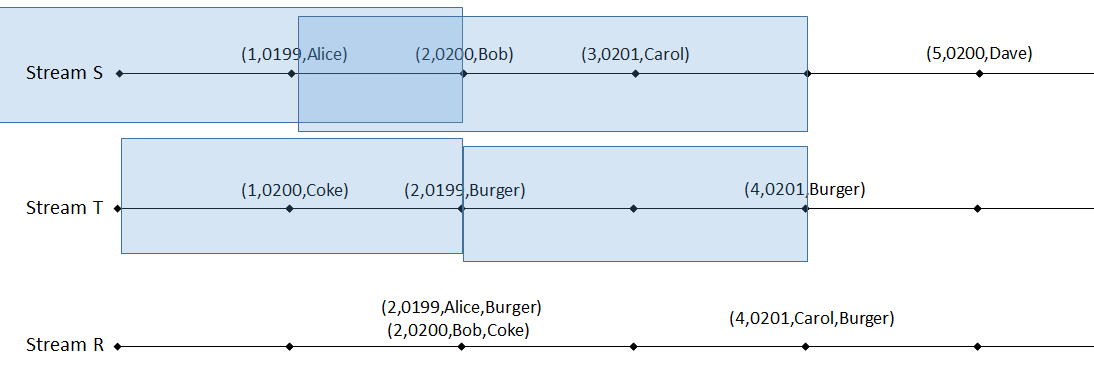
\includegraphics[width=5in]{intro-example}
\caption{Sliding-window JOIN over two in-order data streams \label{fig:intro-example}}
\end{figure}

In many scenarios, the temporal order in which tuples arrive are not the same as the order in which they are generated at data sources, due to unpredictable network behavior. An example is shown in Figure \ref{fig:intro-example-ooo}. This is the case especially when the SPE and the data sources are in a distributed environment. Tuple (1, 0200, Coke) from Stream T' will be discarded when it arrives at the SPE, because it is already late for the window (3, 5]. This leads to the loss of the result tuple (2, 0200, Bob, Coke).\\

\begin{figure}[h]
\centering
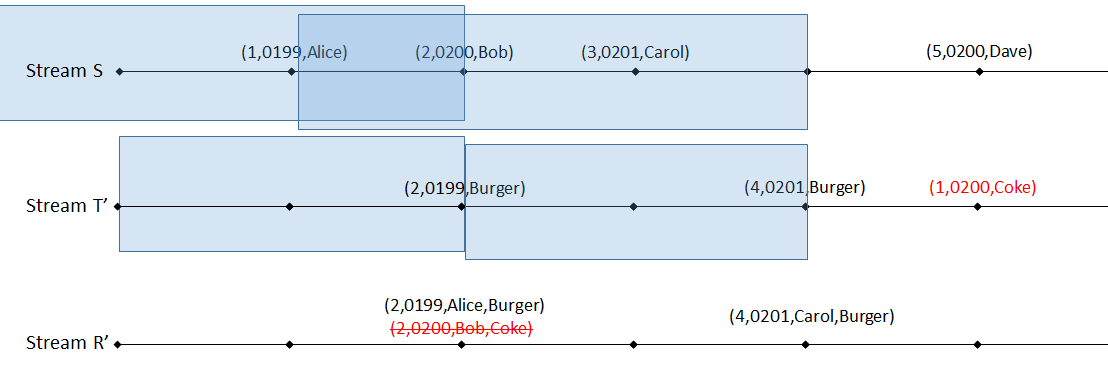
\includegraphics[width=5in]{intro-example-ooo}
\caption{Sliding-window JOIN over out-of-order data streams \label{fig:intro-example-ooo}}
\end{figure}

In order to keep the original semantics of the query, different disorder handling approaches have been proposed \cite{Babu:2004:EKC:1016028.1016032}\cite{barga2006consistent}\cite{Srivastava:2004:FTM:1055558.1055596}. They can increase result latency to improve the result quality\footnote{See details in Chapter \ref{chapter:related-work}.}.\\

\begin{comment}
  trade  Figure \ref{fig:before_and_after_k_slack} shows the two original out-of-order streams and the corresponding in-order streams after applying a buffer based \textit{K}-Slack \cite{Babu:2004:EKC:1016028.1016032} disorder handling approach.\\

\begin{figure}[h]
\centering
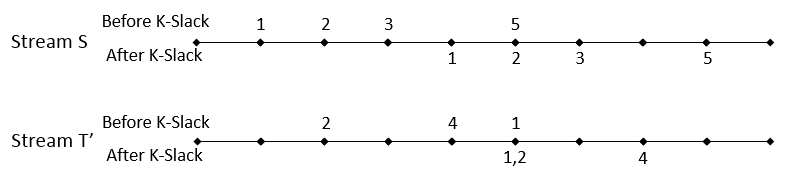
\includegraphics[width=5in]{intro-afterslack}
\caption{Data Stream S and T'(before and after \textit{K}-Slack) \label{fig:before_and_after_k_slack}}
\end{figure}

A \textit{K}-Slack with a buffer of 3 seconds is applied for each input stream. That means, a tuple with timestamp $ts$ will stay in the buffer until the global time reaches  $ts+3$, waiting for potential late tuples. From the figure we can see that with the penalty of waiting for additional 3 seconds, the SPE can process as if there were no disorder in Stream T' and produce result in the same way in the first example.\\

The example above suggests that one must increase result latency to improve the result quality. 
\end{comment}

Motivated by the fact that many applications can tolerate small incorrectness of the result while having high requirement on the result latency \cite{abadi2003aurora}, \textit{quality-driven} disorder handling approaches are proposed, which allow user to specify an expected quality of the result, to speed up the stream processing \cite{Lisa}. In this thesis, we follow the quality-driven disorder handling path and focus on the \textit{sliding-window} JOIN operation.\\

The contributions of this work are as follows. Using the state-of-the-art quality metric for data stream JOIN operation, we propose a probabilistic model to reveal the relationship between buffer size and result quality, when the late arrival pattern of the incoming stream data are observed. We implement the buffer size adaptation logic utilizing this model to minimize the result latency while fulfilling users' requirement on result quality. We have experimentally validated the effectiveness of our adaptation method with real-world stream data and compared it with other adaptation methods.\\

The rest of the thesis is organized as follows. We first introduce the preliminaries in Chapter 2 and discuss the related work in Chapter 3. Secondly, we formally describe our system model in Chapter 4. In Chapter \ref{chapter:quality-driven}, we introduce our probabilistic-based model and concentrate to describe our quality-driven adaptation algorithm. We present the implementation of our proposal and the experimental evaluation in Chapter 6. Finally, we conclude in Chapter 7.\\

\cleardoublepage


\chapter{Preliminaries}
In this chapter, we describe the preliminaries. We explain our time model, stream model and window model respectively.\\

\section{Time Model}
In this thesis, we assume that the local clocks at all data sources and at the data stream processor are always accurate and synchronized\footnote{Nowadays, we can achieve this using GPS clocks, the Network Time Protocol, etc.}.\\

\textbf{\textit{Definition 1 (Application Timestamp)}} The timestamp which is assigned to each tuple according to the local clock at the data source when the tuple is generated, is called an application timestamp.\\

\textbf{\textit{Definition 2 (System Timestamp)}} The timestamp which is assigned to each tuple according to the local clock at the data stream processor when the tuple arrives, is called a system timestamp.\\

Since there is only one clock at the data stream processor, system timestamps are always monotonically increasing. Therefore discussing disorder handling based on system time is meaningless. A tuple's application timestamp is not necessarily the same as, and is usually smaller than, its system timestamp, due to many reasons like network delay. This introduces the disorder problem. We will use application timestamps in the remainder of this work unless stated specifically.\\

\section{Stream Model}

In this thesis, we adopt a similar stream model as defined in \cite{Cormode:2008:TAO:1376916.1376930}:\\

\textbf{\textit{Definition 3 (Stream)}} A data stream is an (unbounded) sequence of tuples $e = (e.v, e.ts)$, where $e.v$ is the value of the tuple and $e.ts$ is the timestamp of the tuple.\\

\textbf{\textit{Definition 4 (Out-of-order Stream)}} An out-of-order stream is a stream which contains at least one out-of-order tuple. An out-of-order tuple is a tuple that arrives later (has a greater system timestamp) than any tuple with a bigger application timestamp. Any other tuples are in-order tuples. Formally, Stream $S$ is an out-of-order stream, iff
\begin{center}
$\exists e_i, e_j \in S$, where $e_i.ts > e_j.ts\ \wedge\ e_i.ts_{sys} < e_j.ts_{sys}$\\
\end{center}

The \textit{in-order substream} for an out-of-order stream S is a stream which excludes all out-of-order tuples in S.\\

\textbf{\textit{Definition 5 (Stream Group)}} A stream group is a group of at least two streams. It can be merged into a $merged$ stream with the ascending order of system timestamps.\\

\textbf{\textit{Definition 6 (Out-of-sync Stream Group)}} A stream group is out-of-sync, if the merged stream of the in-order substreams of all its streams is an out-of-order stream.\\

\textbf{\textit{Definition 7 (Out-of-order Stream Group)}} An out-of-order stream group is a stream group whose merged stream is an out-of-order stream. It can be due to any of out-of-order stream in the group, or out-of-sync between streams.\\

\section{Window Model}

In order to limit the scope of interest over a potentially infinite stream, the concept of \textit{window} has been proposed \cite{abadi2005design}. A window is a consecutive subset of a stream. Operations are applied upon the tuples within a window instead of within the whole stream. A window can have a size $W$, which can be either time-based (e.g., 5 seconds), or tuple-based (e.g., 10 tuples). We use the same definitions of time-based window and  defined in \cite{ayad2004static}.\\

\nomenclature{$W$}{The size of a window}%

\textbf{\textit{Definition 8 (Time-based Window)}} At any time instant $t$, a time-based
window of size $W$ on a stream S defines a subset of S containing all elements of S with timestamp $ts$ such that $t-ts\leq W$.\\

\textbf{\textit{Definition 9 (Tuple-based Window)}} At any time instant $t$, a tuple-based
window of size $W$ on a stream S defines a subset of S with the largest $W$ timestamps not exceeding $t$. If the size of S at time $t$ is less than $W$, the window includes all elements of the stream.\\

In this thesis we focus on time-based windows, and our approach is extensible for tuple-based windows.\\



The window moves forwards as new tuples come. Time-based windows can move in two ways, tumbling and sliding \cite{patroumpas2006window}. Figure \ref{fig:sliding_window} gives an example for these two types of windows. A time-based sliding window each time moves a fixed length, which is defined as \textit{window slide unit} (notated as $U$). A tumbling window can be considered as a sliding window with $U=W$.\\

\nomenclature{$U$}{Window slide unit}%

\begin{figure}[h]
\centering
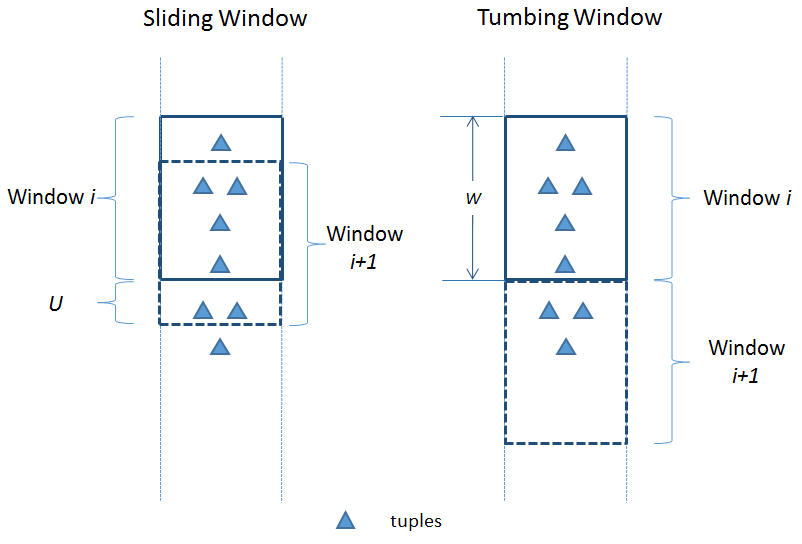
\includegraphics[scale=0.6]{sliding-window}
\caption{Sliding window versus tumbling window \label{fig:sliding_window}}
\end{figure}

Apply tumbling windows on two input streams with different window sizes, will result in two streams out-of-sync, because the stream with smaller window size always moves slower than the one with larger window size. In this thesis, we allow streams with different window sizes. Therefore, we discuss sliding windows.\\

We summarize important notations used in this thesis on Page \pageref{nomenclature}.

\cleardoublepage

\chapter{Related Work}
\label{chapter:related-work}

In recent years, several works have addressed the disorder handling problem in data stream processing. In this chapter, we briefly introduce the ways that they handle the intra-stream disorder problem in Section \ref{subsec:intra-stream disorder handling}, and the inter-stream disorder problem in Section \ref{sec:inter-stream disorder handling}. We then give a short summary in Section \ref{sec:summary-intrastream}.\\

\section{Intra-Stream Disorder Handling}
\label{subsec:intra-stream disorder handling}
Aiming to solve the out-of-order problem within an individual stream, a variety of approaches have been proposed. In this section, we demonstrate buffer-based approaches (Section~\ref{subsec:buffer based approaches}), punctuation-based approaches (Section~\ref{subsec:punctuation based approaches}), speculation-based approaches (Section~\ref{subsec:speculation based approaches}), and a hybrid approach combining buffering and speculation (Section \ref{subsec:hybrid approaches}).\\

\subsection{Buffer-Based Approaches}
We first look at the buffer-based disorder handling approaches. Buffer-based approaches use buffers to handle the disorder problem. We will take the out-of-order stream S in Figure \ref{fig:input} as input stream for all examples in this section. Tuples are notated as $ei$ where $i$ represents the timestamp of the tuple. For instance, $e1$ denotes a tuple with timestamp 1.\\

\begin{figure}[h]
\centering
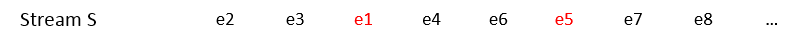
\includegraphics[width=5in]{input}
\caption{Stream S ($e1$ and $e5$ are out-of-order)\label{fig:input}}
\end{figure}

\label{subsec:buffer based approaches}

\noindent\textbf{Static \textit{K}-Slack Approach}\\

Babu et al. \cite{Babu:2004:EKC:1016028.1016032} have introduced the concept of \textit{k-constraints}, which is later often referred to as \textit{K}-Slacks. A $slack$ is a buffer that can temporarily store and sort incoming tuples. The $clk$ is defined as the largest timestamp that is ever observed in a stream. With a predefined parameter \textit{K}, the slack stores all tuples with a timestamp within the time interval (\textit{clk-K}, \textit{clk}], and releases all tuples with a timestamp smaller than or equal to \textit{clk-K} in ascending order of timestamps. \\

\noindent\textbf{\textit{Example}} Figure \ref{fig:statik-k-slack-example} gives an example how the static \textit{K}-Slack approach is used to handle the out-of-order Stream S. When out-of-order tuple $e1$ comes, \textit{clk} is 3, the slack is buffering $e2$ and $e3$. Since $1\not\in(clk-K, clk]$, $e1$ does not go into the slack but goes directly to the output. Afterwards, $e4$ comes and updates \textit{clk} to 4, so that $e2$ can be released. Similarly, the slack releases $e5$ when $e7$ comes. The output stream of \textit{K}-slack is in-order.\\

\begin{figure}[h]
\centering
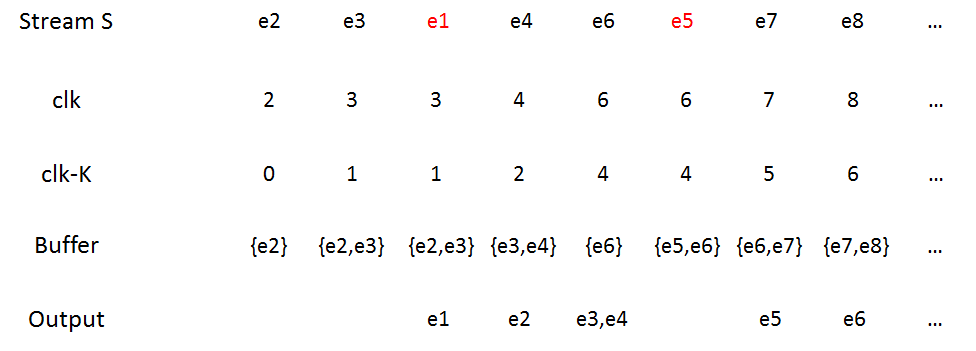
\includegraphics[width=5in]{statik-k-slack-example}
\caption{Static \textit{K}-Slack Approach (K=2) \label{fig:statik-k-slack-example}}
\end{figure}

From this example we can see that, a \textit{K}-Slack with a static size of 2 time units can tolerate tuples which are delayed by at most 2 time units. If $e1$ comes after $e4$ (delayed by 3 time units), then $e2$ will be before $e1$ even if in the output of \textit{K}-Slack. As a concequence, it causes that the processing of each in-order tuple is delayed by at least 2 time units\footnote{Tuple $e3$ is delayed by 3 time units. This is because in the model of Babu et al., the slack can only "infer" the "current global time" from the largest observed timestamp(\textit{clk}). And since $e5$ is late, it does not update \textit{clk} until $e6$ comes.}.\\

\noindent\textbf{Adaptive \textit{K}-Slack approach}\\

In the static \textit{K}-slack approach, the parameter \textit{K} is chosen in advance and stays invariant during the processing. Therefore, a-priori knowledge of the incoming stream data is required. An improperly chosen \textit{K} may lead to either a still-not-in-order output stream, if \textit{K} is too small; or a huge result latency, if \textit{K} is too large.\\

Aiming to overcome this drawback, Mutschler et al. \cite{10.1109/IPDPS.2013.29} propose the adaptive \textit{K}-slack approach, in which \textit{K} is initialized to 0 and is dynamically adjusted according to the runtime measurement of the tuple delays ($clk-e.ts$). This means that no a-priori knowledge is required. \\

\noindent\textbf{\textit{Example}} Figure \ref{fig:adaptive-k-slack-example} gives an example of the adaptive \textit{K}-Slack approach. \textit{K} is initialized to 0. When $e1$ comes, \textit{K} is still 0 because there have been no out-of-order tuples. At this moment, an out-of-order $e1$ in the output of \textit{K}-Slack is inevitable, because $e2$ and $e3$ have already been released. \textit{K} is updated to 2, because $e1$ is late for 2 time units. Any future tuples late for no more than 2 time units will be tolerated, like $e5$. A future tuple which is late for more than 2 time units will still be an out-of-order tuple in the output of \textit{K}-Slack and will update \textit{K} in the meantime.\\

\begin{figure}[h]
\centering
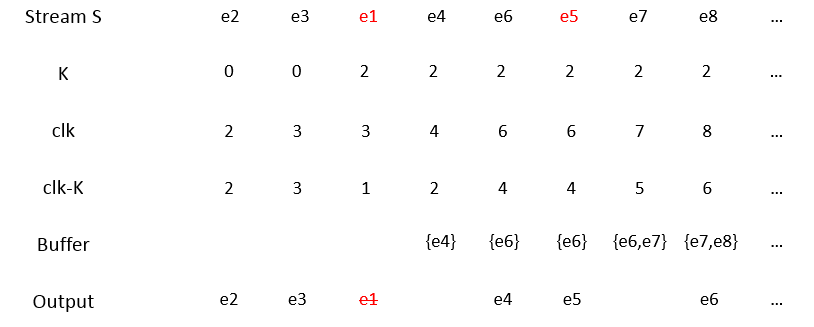
\includegraphics[width=5in]{adaptive-k-slack-example}
\caption{Adaptive \textit{K}-Slack approach \label{fig:adaptive-k-slack-example}}
\end{figure}

\noindent\textbf{Quality-Driven Adaptive \textit{K}-Slack Approach}\\

Considering that eventual 100\% correctness of the result is not always required \cite{abadi2003aurora}, Zhou \cite{Lisa} proposes the \textit{quality-driven} adaptive \textit{K}-Slack approach, which extends the original adaptive \textit{K}-Slack approach and can trade the result correctness beyond user's expectation for lower result latency. Figure \ref{fig:lisa_structure} shows the architecture of Zhou's system.\\

\begin{figure}[h]
\centering
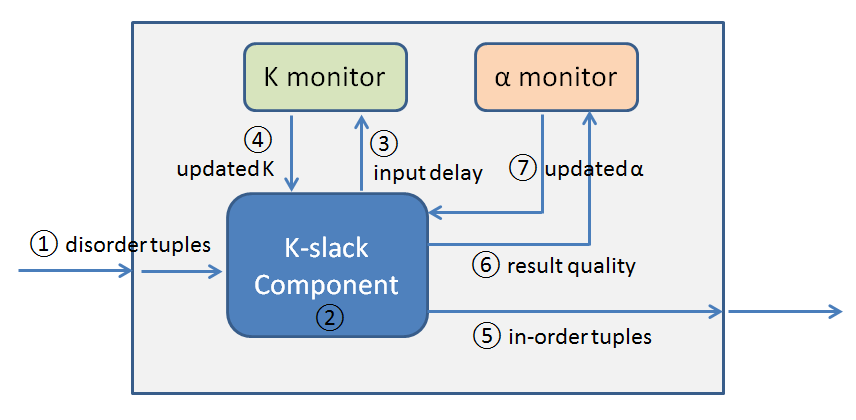
\includegraphics[scale=0.55]{disorder_handling_component_internal_structure.PNG}
\caption{Internal structure of disorder handling component in \cite{Lisa} \label{fig:lisa_structure}}
\end{figure}

Besides $K$ in the original adaptive \textit{K}-Slack approach, Zhou uses an additional parameter $\alpha$ ($\alpha \in [0,1]$), which reduces the buffer size from $K$ to $\alpha K$. Hence, the slack only buffers the tuples with a timestamp within the time duration (\textit{clk-$\alpha K$}, \textit{clk}].\\

In this architecture, the \textit{K}-Slack component not only buffers input tuples, but also tracks the result quality and passes it to the $\alpha$ monitor. Different adaptation algorithms like a PD controller \cite{astrom1995pid} or a TCP controller \cite{Mutschler:2013:RSP:2488222.2488263} can be applied in the $\alpha$ monitor to adjust $\alpha$ according to the current and expected quality values. The updated $\alpha$ is returned to and later applied by the \textit{K}-Slack component. Evaluation results show that a PD controller can achieve a good trade-off between result quality and result latency with proper parameter configuration of the PD controller. Zhou's work only supports aggregation operators currently.\\

\subsection{Punctuation-Based Approaches}
\label{subsec:punctuation based approaches}

Tucker \cite{tucker2005punctuated} first uses $punctuations$ to deal with the disorder problem in data stream processing. Punctuations are special tuples embedded in a data stream that mark the end of substreams. Punctuations can be generated in different places, such like at data sources \cite{tucker2005punctuated}\cite{abadi2003aurora}, at middlewares \cite{krishnamurthy2010continuous}, or in the SPE \cite{li2005semantics}. Figure \ref{fig:punctuation-base} shows an example, in which punctuations are provided by an input manager \cite{krishnamurthy2010continuous}.\\

\begin{figure}[h]
\centering
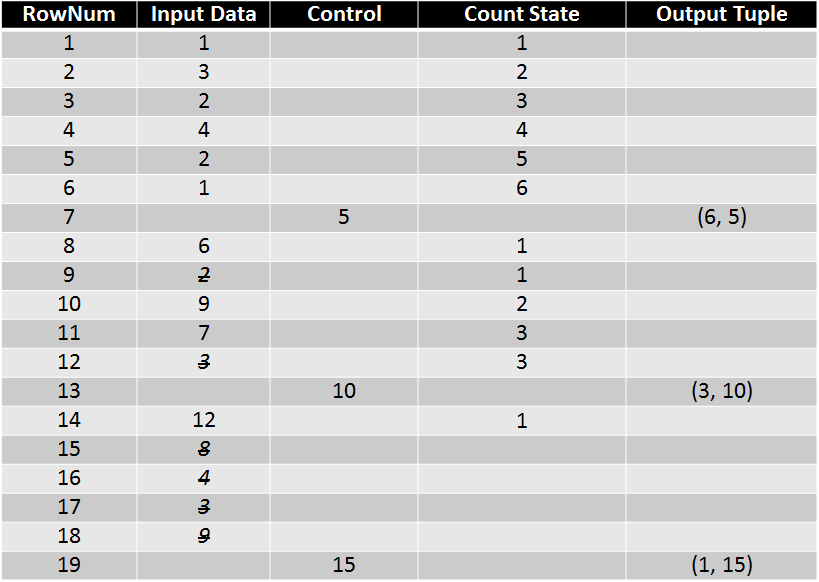
\includegraphics[scale=0.55]{punctuation-base}
\caption{Punctuation-based disorder handling \cite{krishnamurthy2010continuous} \label{fig:punctuation-base}}
\end{figure}

In this example, the SPE counts the number of tuples within a tumbling window with a size of 5 time units. This means it outputs the result at the end of every 5 time units. The column \textbf{Input Data} shows the original timestamps of tuples. The column \textbf{Control} shows the punctuation tuples generated by the input manager based on some heuristic. The SPE records counting result as \textbf{Count State} internally, and outputs it as \textbf{Output Tuple} once receiving a punctuation tuple.\\

More specifically, from Row 1, the SPE counts every input tuple. In Row 7, the punctuation with timestamp 5 indicates that the window $(0,5]$ is end. Therefore, at this moment the SPE is safe to output a result (6,5) and reset the counter to 0. Since then, any Input Data  tuple with a timestamp not larger than 5 (like in Row 9 or in Row 12) is discarded. In Row 13 comes another punctuation with timestamp 10, which ends the window $(5,10]$.

\subsection{Speculation-Based Approaches}
\label{subsec:speculation based approaches}

In speculation based approaches, the SPE assumes that input is in-order and does not wait for late arrivals. When a late tuple arrives, the system will invalidate early results which are affected by the late arrival, and produce an updated result by replaying the stream from the late tuple's timestamp to correct the result \cite{barga2006consistent}.\\

\noindent\textbf{\textit{Example}} Figure \ref{fig:speculation-based-example} demonstrates an example using speculation-based approach. The SPE counts the number of tuples within a tumbling window with a size of 2 time units. When $e3$ arrives, the system will output the result $count([1,2])=1$, since the window [1,2] is over. When the out-of-order tuple $e1$ arrives, the SPE knows the previous result was wrong, hence reproduce a new correct result $count([1,2])=2$. Not all out-of-order tuples can result in replaying. For example, the out-of-order tuple $e5$ does not cause replaying, because it does not invalidate any previous results.\\

\begin{figure}[h]
\centering
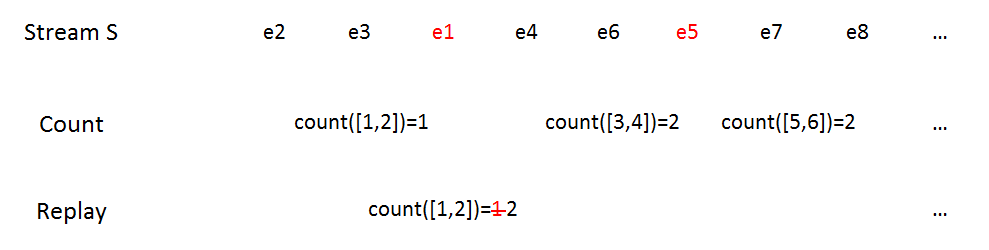
\includegraphics[width=5in]{speculation-based}
\caption{Speculation-based approach\label{fig:speculation-based-example}}
\end{figure}

The speculation based approach is able to provide ``early but conceivably wrong'' results which are valuable in some contexts. It can also achieve eventual correctness with replaying. However, replaying requires additional storage and computation.\\

\begin{comment}
Brito et al. \cite{brito2008speculative} utilize software transactional memory (STM) to achieve eventual correctness. When a tuple comes with a timestamp which is not too early (e.g., advancing more than 10 time units), a $transaction$ is executed and appended to a waiting list. Otherwise it is so early that has a high probability to cause a lot of conflicts, so it will be buffered. If timestamps are supposed to be unique and continuous, the SPE knows exactly which transactions to commit (all before the first missing timestamp). The arrival of the tuple which has the missing timestamp will be committed after execution and trigger a \textit{try-to-commit} chain in the waiting list in timestamp order. Taking advantages of STM, any transaction that has conflicts with its predecessors will fail to commit, thus be rolled back and re-executed.\\

With STM, this approach is able to provide "early but conceivably wrong" results which are valuable in some contexts, without sacrificing eventual correctness. Moreover, STM helps to easily parallelize the event processor, so that the computational latency is reduced due to processing capability increasement. However, the fundamental assumption that timestamps are unique and continuous may not always stand true, without which the event processor will get confused. If there can be multiple tuples with the same timestamp, the event processor will never know whether a tuple with an old timestamp will come or not so it is not able to decide which transactions to commit. If the timestamps are not continuous i.e., some timestamp is missing but the event processor is not aware, then transactions with timestamps after it will stay in the waiting list forever.
\end{comment}

\subsection{Hybrid Approach}
\label{subsec:hybrid approaches}

Experimental evaluations in \cite{10.1109/IPDPS.2013.29} show that the latency is still large even though \textit{K} is determined at runtime. Mutschler et al. \cite{Mutschler:2013:RSP:2488222.2488263} have proposed the speculative \textit{K}-slack approach, which is a combination of the original adaptive \textit{K}-slack approach discussed in Section \ref{subsec:buffer based approaches}, and the specutation-based approach discussed in Section~\ref{subsec:speculation based approaches}.\\

Compared to the original adaptive \textit{K}-slack approach, Mutschler et al. introduce an additional parameter $\alpha (\alpha\in[0,1])$ to reduce the buffer size from $K$ to $\alpha K$. As a result, in speculative \textit{K}-slack approach, the slack only buffers the tuples with a timestamp within the time duration (\textit{clk-$\alpha K$}, \textit{clk}]. Compared to the pure specutation-based approach, this buffer reduces the chance of replaying caused by late arrivals.\\

\noindent\textbf{\textit{Example}} Figure \ref{fig:speculative-k-slack-example} shows an example of speculative \textit{K}-Slack approach with $\alpha=0.5$. The only out-of-order tuple in the output of \textit{K}-Slack is $e1$, which can cause potential replaying. Note that after $e5$, the output is one-time-unit advancing compared with the output in the adaptive \textit{K}-Slack example, because the buffer size is decreased by 1($=(1-\alpha) K$) time unit in the speculative \textit{K}-Slack approach.\\

\begin{figure}[h]
\centering
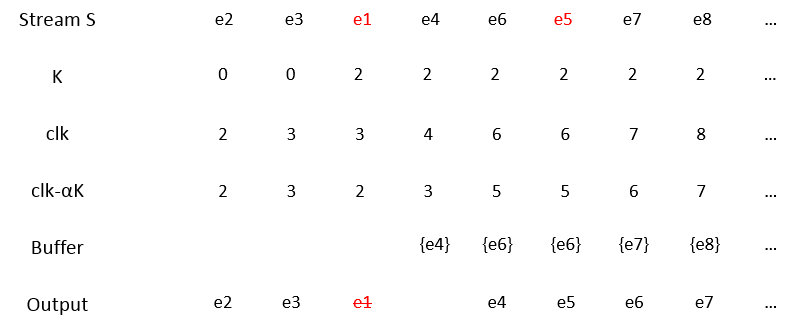
\includegraphics[width=5in]{speculative-k-slack-example}
\caption{Speculative \textit{K}-Slack approach ($\alpha=0.5$)\label{fig:speculative-k-slack-example}}
\end{figure}

Taking advantages of speculation and replaying, the speculative \textit{K}-slack approach can achieve eventual correctness of execution with a smaller buffer size thus lower latency, compared to adaptive \textit{K}-slack approach. The shortcoming is also obvious. Additional storage is required to store released tuples in order to enable replaying. If $\alpha$ is chosen improperly small, replaying may be frequent which causes waste of computation as well as temporarily wrong results.\\

\section{Inter-Stream Disorder Handling}
\label{sec:inter-stream disorder handling}
In data stream processing, when we have operators like JOIN, UNION and INTERSECT, which take more than one streams as input, we must also take inter-stream disorder into consideration, because in a distributed topology it is a trivial situation. Figure \ref{fig:out-of-sync} shows a typical moment when two streams are out-of-sync. Stream B is the leading stream at this moment. The out-of-sync tuples are those tuples that have larger timestamps than any tuple in the lagging stream A.\\

\begin{figure}[h]
\centering
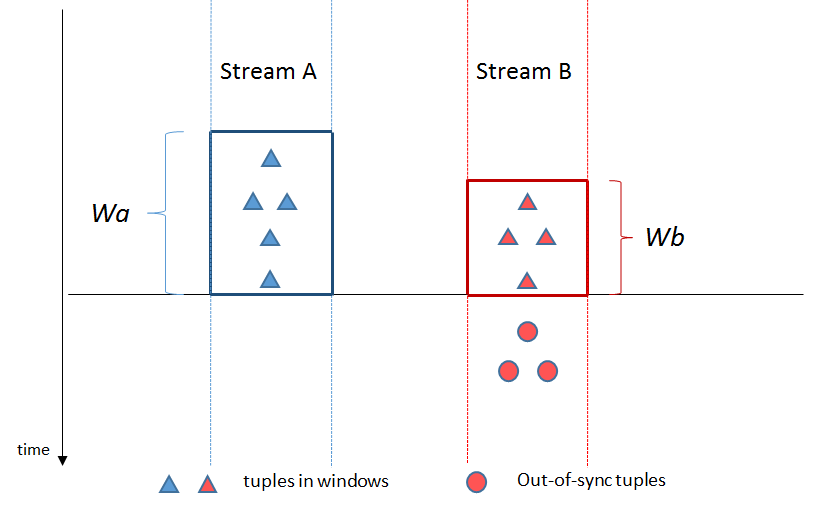
\includegraphics[width=5in]{out-of-sync}
\caption{Out-of-sync streams\label{fig:out-of-sync}}
\end{figure}

Several works have studied how to perform in-order execution over out-of-sync data streams. We describe the Sync-Filter approach, the Filter-Order approach, and deterministic merge in this section. Note for now we only focus on the inter-stream disorder problem, so in this section we assume that there is no intra-stream disorder, i.e., any single stream is in-order.\\

\subsection{Sync-Filter and Filter-Order Approach}
\label{subsec:sync-filter_filter-order}

One straightforward approach, later being referred to as Sync-Filter approach \cite{Hammad05optimizingin-order}, is to buffer the out-of-sync tuples, and produce result based on synchronized input streams at the SPE \cite{Srivastava:2004:FTM:1055558.1055596}.\\

Hammad et al. \cite{Hammad05optimizingin-order} point out that in Sync-Filter approach, the production of result tuples are delayed due to synchronization. For example, in Figure \ref{fig:out-of-sync}, an out-of-sync tuple $b$ in Stream B cannot be joined with any tuple in Stream A at this moment, even though they should be joined according to the semantic of the join query. They can only be joined after Stream A has a tuple $a$ with $a.ts \geq b.ts$, so that $b$ is no longer an out-of-sync tuple. This leads to the processing unit to be idle when streams are waiting for synchronization, and causes a huge overload when streams become synchronized, when all JOIN operations happen.\\

Hammad et al. propose the Filter-Order approach in order to overcome this drawback. In the Filter-Order approach, tuples can be joined when they arrive at the SPE. However, this will lead to an out-of-order output stream. Thus, an output buffer is used to temporarily store join results. Hammad et al. also give numerical analysis to the average response time of both Sync-Filter approach and Filter-Order approach under different input tuple arrival rates. A threshold is found so that the system is able to switch between Sync-Filter approach and Filter-Order approach to have a better trade-off between memory consumption and response time.\\

\subsection{Deterministic Merge}

Aguilera et al. \cite{Aguilera:2000:EAB:343477.343620} use \textit{deterministic merge} algorithms to ensure multiple $merger$ nodes in a decentralized publish/subscribe system to merge the message streams in exactly the same way, regardless of the delays of messages by the network.\\

\begin{figure}[h]
\centering
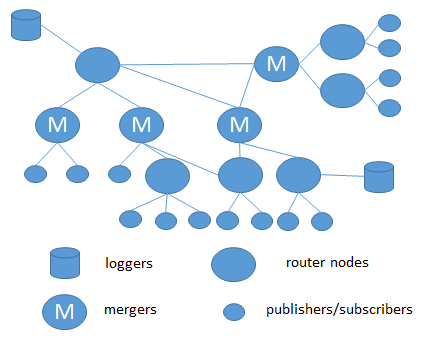
\includegraphics[scale=0.65]{deterministic-merge}
\caption{The architecture of a decentralized publish/subscribe system \cite{Aguilera:2000:EAB:343477.343620}}\label{fig:deterministic_merge}
\end{figure}

As shown in Figure \ref{fig:deterministic_merge}, several subscribers are assigned to one of the mergers. When publishing a message, a publisher first sends it to a logger to log it. Then the logger uses a FIFO link to send this message to any merger that has any subscriber interested it. The deterministic merge algorithm is replicated at every merger node. It can guarantee that all mergers order the messages consistently but independently. One simple deterministic merge algorithm can be that the producers attach timestamps to the messages, and then the mergers order the messages according to the timestamps in ascending order. Better algorithms are proposed in \cite{Aguilera:2000:EAB:343477.343620}.\\

\section{Summary}
\label{sec:summary-intrastream}

For intra-stream disorder handling, the static \textit{K}-Slack approach and the adaptive \textit{K}-Slack approach are good for their simplicity and effectiveness. However, they fail to adjust the buffer size dynamically, to have a trade-off between result quality and result latency according to users' expectation. The quality-driven approach with a PD controller is able to do so, but its performance highly depends on the configuration of parameters \cite{Lisa}. Moreover, it only supports aggregation operations currently. The performance of punctuation-based approaches also depends on the algorithm of generating punctuations. The speculation-based approaches can provide eventual correctness sacrificing additional storage and computation, yet a correct though very late result is arguably meaningless to some applications.\\

For inter-stream disorder handling, the approaches which are discussed in Section \ref{sec:inter-stream disorder handling} all require that each input stream should be in-order. Moreover, there are some additional requirements such like in \cite{Aguilera:2000:EAB:343477.343620}, each producer must be able to estimate all producers' expected message rates.\\

In our work, we consider more general situations for JOIN operation, where streams can be both out-of-order and out-of-sync. Therefore, we must face both intra-stream and inter-stream disorder problem at the same time. We also wish to have a quality-driven approach, so that we can provide result that can meet users' requirement on quality with minimum result latency. We demonstrate our approach in the next chapter.\\


\cleardoublepage

\chapter{System Model}
\label{chapter:system-model}

In this chapter, we demonstrate the system model for sliding window JOIN upon data streams. We first have an overview of our solution, then we explain our join logic in detail.\\

\section{Solution Overview}
\label{sec:solution-overview}

In order to handle the disorder problem and give an in-order result stream for JOIN operation, we adopt a similar system architecture proposed in \cite{wu2007window}.\\

As shown in Figure \ref{fig:system_arch}, one \textit{K}-Slack is applied to each input stream. Their sizes are set to 0 initially and are adjusted at runtime (see Section \ref{sec:adaptation-strategy}). Since the output streams of \textit{K}-Slacks can be potentially out-of-sync, we take the Sync-Filter approach as explained in Section \ref{subsec:sync-filter_filter-order}. A synchronization buffer \textit{SyncBuffer} is used to buffer early tuples in the leading stream in order to wait for tuples in the lagging stream. The \textit{SyncBuffer} is actually a pair of buffers storing early tuples from Stream A and Stream B. We use \textit{SyncBufA} and \textit{SyncBufB} to denote them. The window of the leading side receives synchronized tuples from the \textit{SyncBuffer}, and the window of the lagging side receives tuples directly from the input stream. \\

\nomenclature{\textit{SyncBufA}}{Synchronization buffer of Stream A}%
\nomenclature{\textit{SyncBufB}}{Synchronization buffer of Stream B}%

\begin{figure}[h]
\centering
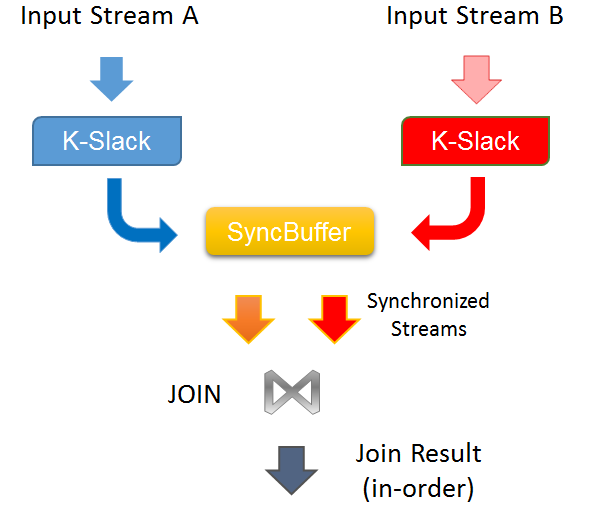
\includegraphics[scale=0.6]{architecture}
\caption{Sliding-window JOIN with disorder handling \label{fig:system_arch}}
\end{figure}

Figure \ref{fig:system_arch_windows} shows the window view at a certain moment. Two windows, the lagging WindowA with size $W_A$, and the leading WindowB with size $W_B$, have the same end point, which equals the smaller one of both streams' maximum timestamp of all arrived tuples. We denote the current common endpoint of both windows as $WindowEnd$. When $WindowEnd$ moves forward, two windows move at the same time. Tuples that have already arrived with timestamps greater than $WindowEnd$ will be pending in \textit{SyncBufA} or \textit{SyncBufB}. There can be at most one nonempty buffer at any point of time. If both buffers are nonempty, $WindowEnd$ will move forward until one buffer is empty.\\

\nomenclature{$WindowEnd$}{Current common endpoint of both windows}%

\begin{figure}[h]
\centering
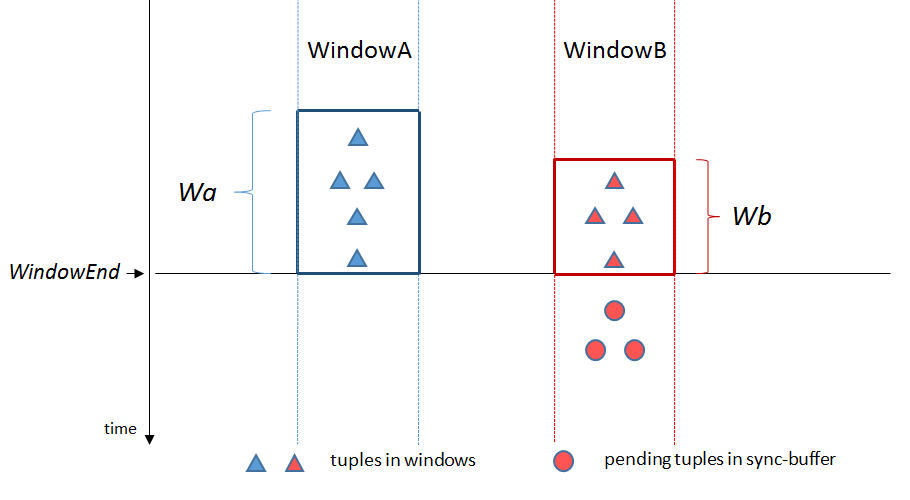
\includegraphics[scale=0.55]{system_arch_windows}
\caption{Sliding-window JOIN with sync-buffer\label{fig:system_arch_windows}}
\end{figure}

For a $sliding$ window, it cannot move if we have not seen not a pending tuple $e$ with $e.ts\geq WindowEnd+U$. So there is a possible counterexample that both windows have pending tuples but $WindowEnd$ does not move, because the windows are not able to slide. For general-case sliding windows, we always wait until the window is able to slide. Right now, for simplicity, we assume that $U$ equals the smallest time unit.\\


\section{Join Logic}

We now explain the detailed join logic.\\

$JOIN(a, b)$ is the JOIN operation applied upon $a$ (a tuple in Stream A) and $b$ (a tuple in Stream B). If the join condition is fulfilled, $JOIN(a, b)$ returns an result tuple $r$ with $r.ts = max(a.ts, a.ts)$; otherwise it returns no result tuple.\\

\nomenclature{$a$}{Input tuples in Stream A}%
\nomenclature{$b$}{Input tuples in Stream B}%
\nomenclature{$r$}{Result tuples in Stream R}%

Since we must guarantee that the result stream is in-order, and there is no extra disorder handling on the result stream, a result tuple $r$ can be released iff $r.ts=WindowEnd$, that is to say, they can only be released when their the timestamp equal to the current end point of the windows. We achieve this by dropping out-of-date result tuples and not generating result tupls ahead of $WindowEnd$. First, if a result tuple $r$ has $r.ts<WindowEnd$ when it is generated, it must be dropped. Otherwise it will lead to the result stream R to be out-of-order. Second, no result tuple r with $r.ts>WindowEnd$ is generated. The JOIN operator waits until $WindowEnd$ moves to $WindowEnd'=r.ts$, and then generate it.\\

From the JOIN operator's perspective, it receives tuples from two \textit{K}-Slacks, which may still be out-of-order due to insufficient buffer size. There are different situations for a newly received tuple $e$. Without losing generality, in this section we assume that tuple $e$ is from Stream A.\\

\noindent\textbf{Situation 1} $e.ts\leq WindowEnd - W_A$\\

In this case, $e$ is too late to be able to contribute to any result tuples $r$ with $r.ts\geq WindowEnd$, so $e$ is simply dropped.\\

\noindent\textbf{Situation 2} $WindowEnd - W_A<e.ts<WindowEnd$\\

In this case, $e$ arrives late but its time stamp is till within the current scope of WindowA, so it is still able to contribute to result tuples $r$ with $r.ts\geq WindowEnd$. The SPE joins $e$ with all tuples $b\in WindowB$ with $b.ts=WindowEnd$, and stores $e$ in WindowA.\\

\noindent\textbf{Situation 3} $e.ts=WindowEnd$\\

In this situation, $e$ is not an out-of-order tuple. Hence, it will be joined with all tuples $b \in WindowB$, and then be stored in WindowA.\\

We demonstrate situation 1, situation 2 and situation 3 in Figure \ref{fig:join_logic_1}.\\

\begin{figure}[!htb]
\centering
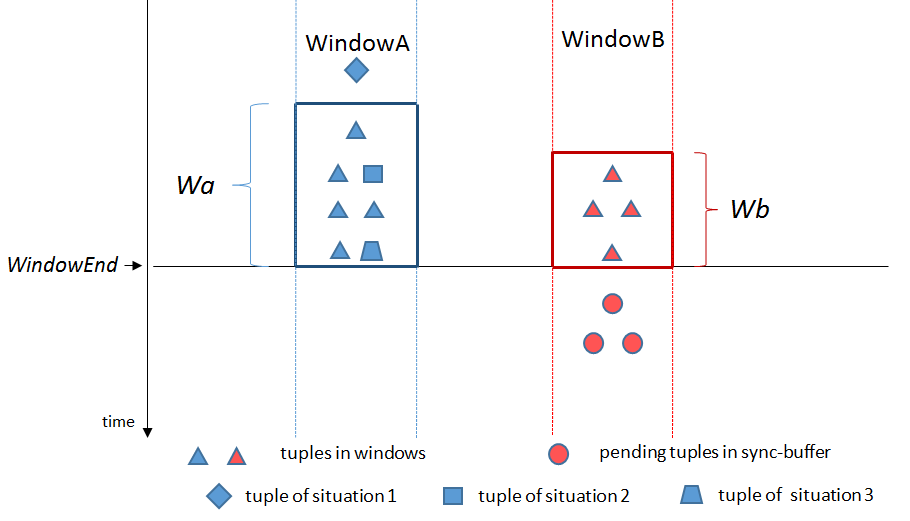
\includegraphics[scale=0.55]{join_logic_1}
\caption{JOIN Logic, different situations\label{fig:join_logic_1}}
\end{figure}

\noindent\textbf{Situation 4} $e.ts>WindowEnd$. There are three sub-situations as follows:\\



\noindent\textbf{Situation 4a} $e.ts>WindowEnd \wedge SyncBufB=\emptyset$.\\

$SyncBufB=\emptyset$ means that Stream B is not the current leading stream (Figure \ref{fig:join_logic_2}). $e$ is simply inserted into \textit{SyncBufA}. At this moment $e$ will not be joined with any tuples, because any result tuple with $e$ as a component will have a timestamp of at least $e.ts$, which is greater than the current $WindowEnd$.\\

\begin{figure}[H]
\centering
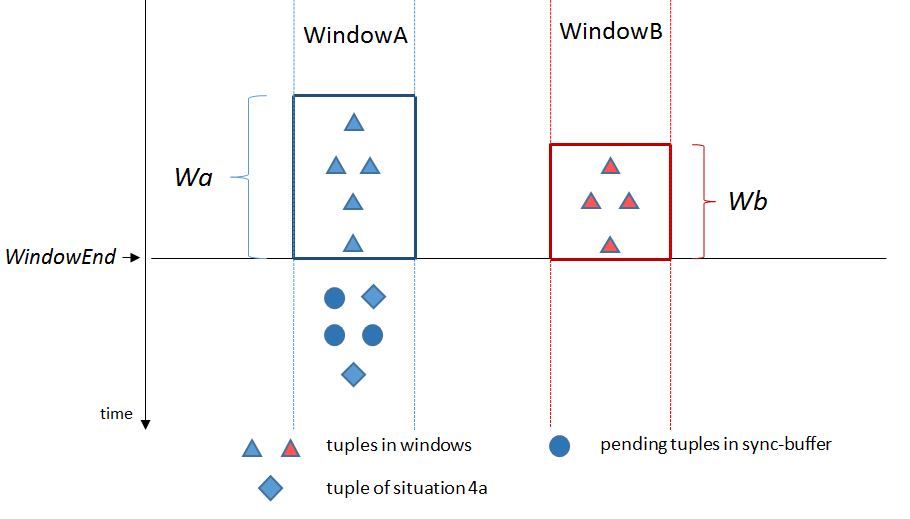
\includegraphics[scale=0.55]{join_logic_2}
\caption{JOIN Logic, Situation 4a\label{fig:join_logic_2}}
\end{figure}

\noindent\textbf{Situation 4b} $e.ts>WindowEnd \wedge SyncBufB\neq \emptyset \wedge e.ts\leq max(b.ts), b \in SyncBufB$\\

$SyncBufB\neq \emptyset$ means that Stream B is the current leading stream. $e.ts\leq max(b.ts), b \in SyncBufB$ means that Stream B will still be leading (Figure \ref{fig:join_logic_3}). In this situation, $WindowEnd$ will be pushed forward, from the smallest timestamp of tuples in \textit{SyncBufB} in ascending order, until $WindowEnd$ reaches $e.ts$ Each movement of $WindowEnd$ triggers a series of actions:

\begin{quote}
1) each window will purge old tuples according to the new $WindowEnd$;
2) newly added tuples to the window will be joined with corresponding tuples.
\end{quote}

Tuple $e$ is the last tuple added to WindowA.\\

\begin{figure}[h]
\centering
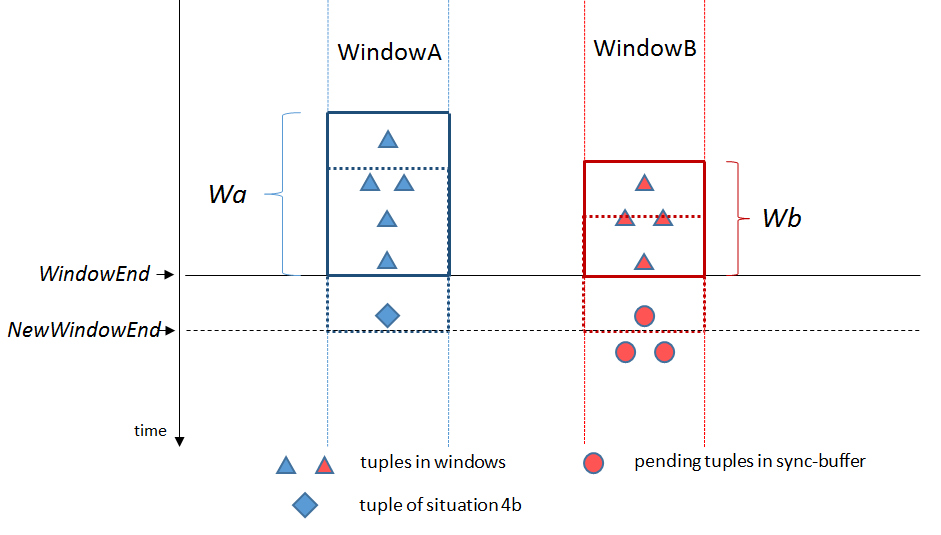
\includegraphics[scale=0.55]{join_logic_3}
\caption{JOIN Logic, Situation 4b\label{fig:join_logic_3}}
\end{figure}

\noindent\textbf{Situation 4c} $e.ts>WindowEnd \wedge SyncBufB\neq \emptyset \wedge e.ts> max(b.ts), b \in SyncBufB$\\

Stream B is the current leading stream, but it will no longer be leading after the window moves. Stream A will become the leading stream, because $e.ts> max(b.ts), b \in SyncBufB$ (Figure \ref{fig:join_logic_4}). The windows move in a similar way as in \textbf{Situation 4b}, but the new $WindowEnd$ will be $max(b.ts), b \in SyncBufB$, and there will be no tuple left in \textit{SyncBufB}. Stream A becomes the leading stream, and $e$ is inserted into \textit{SyncBufA}.\\

\begin{figure}[h]
\centering
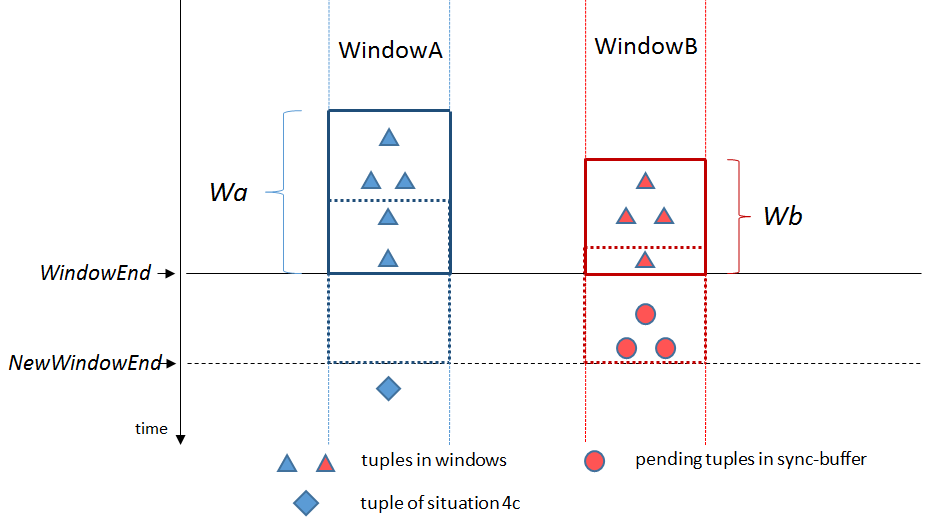
\includegraphics[scale=0.55]{join_logic_4}
\caption{JOIN Logic, Situation 4c\label{fig:join_logic_4}}
\end{figure}

We present the pseudo code of the JOIN logic in Algorithm \ref{algo:join_logic}. In a word, result tuples can only be tagged with the timestamp of the current $WindowEnd$, because we want the result stream to be in-order, and there is no \textit{K}-Slack on the result stream, as we mentioned in the beginning of this section.\\

\clearpage
\begin{algorithm}[H]
\caption{Join Logic\label{algo:join_logic}}
\KwIn{StreamA, StreamB}
\KwOut{StreamR}
$WindowA = \emptyset; WindowB = \emptyset;$\\
$SyncBufA = \emptyset; SyncBufB = \emptyset; WindowEnd = 0$\\
\While{$e \gets getIncomingTuple()$}{
	\eIf{$e \in StreamA$}{
		\uIf{$e.ts \leq WindowEnd - W_A$}{
			drop e;\Comment{Situation 1}
		}
		\uElseIf{$e.ts \leq WindowEnd$}{
			$R \gets$ join $e$ with all $b \in WindowB$;\\
			output $r \in R$, if $r.ts=WindowEnd$, to StreamR;			
			WindowA.insert(e);	\Comment{Situation 2,3}
		}
		\uElseIf{$SyncBufA \neq \emptyset$}{
			\textit{SyncBufA}.insert(e);	\Comment{Situation 4a}
		}
		\Else{
			\While{$\exists b \in SyncBufB, b.ts \leq e.ts$}{
				$b \gets SyncBufB.popTupleWithMinTS();$\\
				$WindowEnd \gets b.ts$;\\
				delete $a \in WindowA$, if $a.ts \leq WindowEnd - W_A$;\\
				$R \gets$ join $b$ with all $a \in WindowA$;\\
				output $r \in R$ to StreamR;\\
				WindowB.insert(b);		\Comment{lazy retention here}
			}
			\eIf{$SyncBufB \neq \emptyset || e.ts == WindowEnd$}{
				$WindowEnd \gets e.ts$;\\
				delete $a \in WindowA$, if $a.ts \leq WindowEnd-W_A$;\\
				delete $b \in WindowB$, if $b.ts \leq WindowEnd-W_B$;\\
				$R \gets$ join $e$ with all $b \in WindowB$;\\
				output $r \in R$ to StreamR;\\
				WindowA.insert(e);	\Comment{Situation 4b}
			}{				
				delete $b \in WindowB$, if $b.ts \leq WindowEnd-W_B$;\\
				\textit{SyncBufA}.insert(e);	\Comment{Situation 4c}
			}
		}
	}{
		do similar;\Comment{$e \in StreamB$}
	}
   }
\end{algorithm}









\cleardoublepage



\chapter{Quality-Driven Slack Size Adaptation}
\label{chapter:quality-driven}

In this chapter, we demonstrate our approach to adjust the \textit{K}-Slack buffer size in order to meet the users' requirement on the join result quality. In Section \ref{sec:quality-metric}, we introduce the formal definition of result quality. In Section \ref{sec:late-degree-distribution}, we introduce the concept of late degree distribution. In Section \ref{sec:quality-estimation}, we reveal the relationship among late degree distributions, buffer sizes and the result quality. We also manage to estimate the result quality if the other two are known. In Section \ref{sec:adaptation-strategy}, we discuss the detailed slack size adaptation approach based on the conclusion of Section \ref{sec:quality-estimation}.

\section{Quality Metric}
\label{sec:quality-metric}
It is important to have a quantitative indicator to demonstrate how good a join result set is. According to Algorithm \ref{algo:join_logic} in Chapter \ref{chapter:system-model}, late arrived input tuples can cause missing of result tuples. However, they do not have any side effect on the other results. In other words, there are never ``bad results'' produced because of late arrived input tuples. Therefore, the quality of a join result set over a period of time can be defined as the number of result tuples that are $actually\ produced$ within this period of time (notated as $Nr_{produced}$), divided by the number of result tuples that $should\ be\ produced$ within this period of time, if there is no disorder in input streams (notated as $Nr_{original}$). Formally, we define the result quality of a join result set, denoted by $Q$, as in \cite{wu2007window}:

\begin{equation}
\label{eq:quality}
Q = \frac{Nr_{produced}}{Nr_{original}}\times 100\%
\end{equation}

\nomenclature{$Q$}{Result quality}%

\nomenclature{$Nr_{produced}$}{The number of result tuples that are actually produced over a period of time}%
\nomenclature{$Nr_{original}$}{The number of result tuples that should be produced over a period of time, if there is no disorder in input streams}%

In general, the fewer missing result tuples we have, the better the result quality we achieve. When no input tuple arrives late, the number of result tuples we actually produce is equal to the number of original results, so the quality would be 100\%. Since by no means can we produce more result tuples than the complete result set, the quality can never surpass 100\%.

\section{Late Degree Distribution}
\label{sec:late-degree-distribution}

We use a late degree distribution $D$ to describe the disorder pattern of an out-of-order stream within a time interval. A late degree distribution $D$ is a probability distribution, describing the pattern of arrival times of input tuples in the stream. The late degree distribution of a stream S can be denoted as:

$$D_S = \{p_{S0}, p_{S1}, p_{S2}, ..., p_{S\Lambda_{max}}\}, sum(p_{S\Lambda})=1$$

$\Lambda$ represents the late degree of an input tuple. If an input tuple $e$ has a timestamp $e.ts$ not smaller than the largest timestamp that has been processed when $e$ arrives (notated as $e.ts_{process}$), then $\Lambda=0$; if $e$ has a timestamp $e.ts$ smaller than $e.ts_{process}$, then it has a late degree $\Lambda=e.ts_{process}-e.ts$. For a single stream with no \textit{K}-Slack, $e.ts_{process}$ equals the maximum observed timstamp $clk$ when $e$ arrives. For the join logic we proposed in Algorithm \ref{algo:join_logic}, $e.ts_{process}$ equals the $WindowEnd$ when $e$ arrives.\\

$p_{S\Lambda}$ represents the probability that a tuple has a late degree of $\Lambda$. Exceptionally, $p_{S\Lambda_{max}}$ represents the probability that a tuple has a late degree of $\Lambda_{max}$ or more. The sum of all $p_{S\Lambda}$ should be 1. We can observe empirical probabilities for all $\Lambda$ by recording $\Lambda$ of each tuple before the \textit{K}-Slack (see Section \ref{subsec:late-degree-monitor} for detail), thereby estimate each value in $D_S$.\\

Figure \ref{fig:late_degree_distribution} shows a possible late degree distribution $D_S = \{p_{S0}=0.6, p_{S1}=0.2, p_{S2}=0.1, p_{S3}=0.1\}$. Based on this distribution we can say that, for an input tuple $e$ in Stream S, the probability that it arrives on time (with $e.ts$ equal to the $clk$ \textbf{of the moment it arrives}) is 60\%; the probability that it is delayed by 1 time unit (with $e.ts=clk-1$) is 20\%; the probability that it is delayed by 2 time units (with $e.ts=clk-2$) is 10\%; the probability that it is delayed by not less than 3 time units (with $e.ts\geq clk-3$) is 10\%.\\

\nomenclature{$D_S$}{Late degree distribution of Stream S}%
\nomenclature{$e.ts_{process}$}{The largest timestamp that has been processed when $e$ arrives}%
\nomenclature{$\Lambda$}{Late degree of a tuple}%

\begin{figure}[h]
\centering
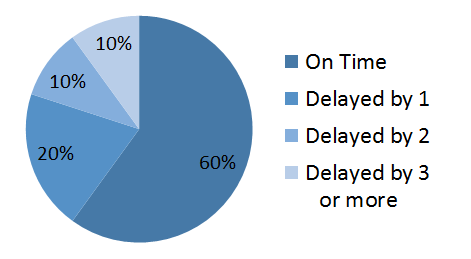
\includegraphics[scale=0.75]{late_degree_distribution}
\caption{Example of late degree distribution $D_S$\label{fig:late_degree_distribution}}
\end{figure}

If $D_S$ is considered constant within a short period of time (in this example 4 time units), we can go one step further, deriving that for an input tuple $e$ in Stream S, the probability that it arrives before $clk$ reaches $e.ts+1$ is 60\%; the probability that it arrives before $clk$ reaches $e.ts+2$ is 80\%(=60\%+20\%); the probability that it arrives before $clk$ reaches $e.ts+3$ is 90\%(=60\%+20\%+10\%). (Figure \ref{fig:total-arrived-tuples})\\

\begin{figure}[h]
\centering
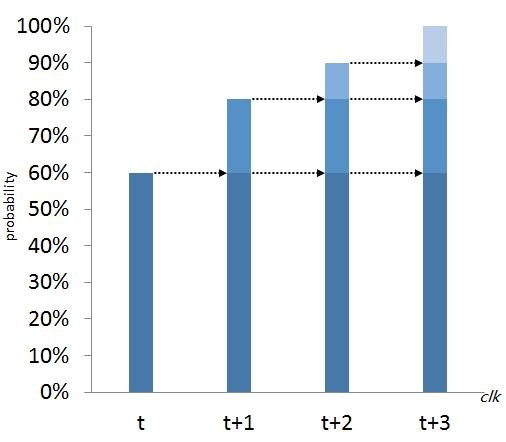
\includegraphics[scale=0.75]{total-arrived-tuples}
\caption{Arrived time probability\label{fig:total-arrived-tuples}}
\end{figure}

Now we consider reversely. At the moment that $clk$ increases from $t$ to $t+1$, for a tuple $e$ with $e.ts=t$, the probability that $e$ has arrived is 60\%; for $e$ with $e.ts=t-1$, the probability that $e$ has arrived is 80\%; for $e$ with $e.ts=t-2$, the probability that $e$ has arrived is 90\%.\\

\subsection{Transformation of Late Degree Distributions}

Applying \textit{K}-Slack on the input stream will change the late degree distribution. For example, consider that applying a static \textit{K}-Slack with a size of 1 time unit. This will allow all in-order input tuples delayed by 1 time unit to be reordered by the K-slack buffer and output in correct order (see Section \ref{subsec:buffer based approaches}), which means for all input tuples $e$, we have $e.ts^{\prime}_{process}=e.ts_{process}-1$. Hence,

\begin{quote}
	a) For those tuples that had $\Lambda = 0$, they will remain on time;

	b) For those tuples that had $\Lambda > 0$, they will have a late degree after \textit{K}-Slack $\Lambda^{\prime}$ with $\Lambda^{\prime}=\Lambda-1$.\footnote{Since $\Lambda=e.ts_{process}-e.ts$, and $\Lambda^{\prime}=e.ts^{\prime}_{process}-e.ts=e.ts_{process}-1-e.ts=\Lambda-1$.}
\end{quote}

Therefore, the late degree distribution (shown in Figure \ref{fig:late_degree_distribution2}) for the output stream of the aforementioned static \textit{K}-slack with a size of 1 time unit, denoted as $D_S^{\prime}$, can be calculated as:

$$D_S^{\prime}(K=1)=\{p^{\prime}_{S0}=p_{S0}+p_{S1}=0.8, p^{\prime}_{S1}=p_{S2}=0.1, p^{\prime}_{S2}=p_{S3}=0.1\}$$\\

More generally, we could derive the late degree distribution after applying a \textit{K}-Slack with a size of $K$ time units:

\begin{equation}
\begin{split}
D_S^{\prime}(K)=\{p^{\prime}_{S0}= \sum\limits_{i=0}^{K} p_{Si}, p^{\prime}_{S\Lambda}=p_{S(K+\Lambda)}, ..., p^{\prime}_{S(\Lambda_{max}-1)} = p_{S\Lambda_{max}}\},	\\
(0 < \Lambda \leq \Lambda_{max}-K)
\end{split}
\end{equation}

\begin{figure}[h]
\centering
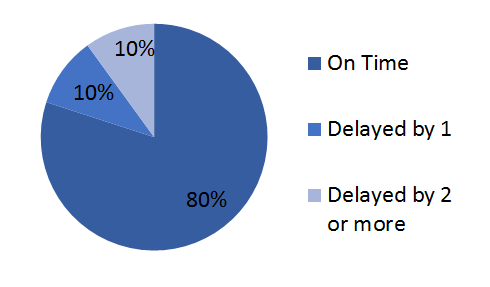
\includegraphics[scale=0.75]{late_degree_distribution2}
\caption{Late degree distribution $D_S^{\prime}$ of the output stream of \textit{K}-Slack \label{fig:late_degree_distribution2}}
\end{figure}

Similarly, \textit{SyncBuffer} also changes the late degree distribution, since applying a \textit{SyncBuffer} with a size of $L$ time units will also make the processing of all in-order input tuples delayed by $L$ time units, which means for all input tuples $e$, we have $e.ts^{\prime}_{process}=e.ts_{process}-L$. In general, if an out-of-order stream S has a \textit{K}-Slack with size $K$ and a \textit{SyncBuffer} with size $L$, its original late degree distribution $D_S= \{p_{S0}, p_{S1}, p_{S2}, ..., p_{S\Lambda_{max}}\}$ will be transformed to:

\begin{equation}
\label{eq:distibution_transform}
\begin{split}
D_S^{\prime}(K,L)= \{p^{\prime}_{S0}= \sum\limits_{i=0}^{K+L}p_{Si}, p^{\prime}_{\Lambda}=p_{S(K+L+\Lambda)}, ..., p^{\prime}_{S(\Lambda_{max}-1)} = p_{S\Lambda_{max}}\}, \\
(0 < \Lambda \leq \Lambda_{max}-K-L)
\end{split}
\end{equation}

\nomenclature{$K$}{Size of a \textit{K}-Slack}%
\nomenclature{$L$}{Size of \textit{SyncBuffer}}%

\section{Quality Estimation}
\label{sec:quality-estimation}

Now we present how we estimate the result quality of the JOIN operation within a time interval $T$ which contains $n$ time units. If $T$ is short enough, we can consider that the data rates and the late degree distributions of both streams, as well as the join selectivity are stable (see discussions in Section \ref{subsec:estimation-of-quality}). We denote the number of tuples with each timestamp in both streams as $n_{A}$ or $n_{B}$, and the join selectivity as $\rho$.\\

To help explain the key idea of our solution, we give an example, in which we join two streams A and B with window slide unit $U=1$ time unit. To ease the presentation, we assume that both streams have the same late degree distribution $D$ as shown in Figure \ref{fig:late_degree_distribution}. We also assume that the two streams are in-sync, and no \textit{K}-Slack is applied. We will relax these assumptions and discuss the general case in Section \ref{subsec:generalization-quality-estimation}.\\

\begin{figure}[h]
\centering
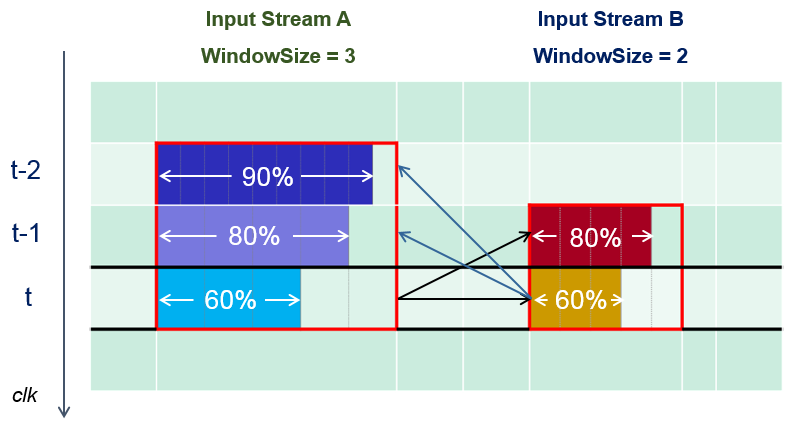
\includegraphics[scale=0.6]{quality-estimation}
\caption{Quality estimation for $t$\label{fig:quality-estimation}}
\end{figure}

\subsection{Estimation of \textit{Nr\textsubscript{original}}}

We now demonstrate how we estimate $Nr_{original}(t)$ for any time unit $t$ in $T$.\\

\nomenclature{$Nr_{original}(t)$}{The number of original result tuples for the time unit $t$}%

A result tuple $r$ with timestamp $r.ts=t$ can be produced as a result of either a tuple $a$ from Stream A with $a.ts=t$, or a tuple $b$ from Stream B with $b.ts=t$, or both of them. Therefore, $Nr_{original}(t)$ contains four parts:

\begin{quote}
 Part 1. $a$ with $a.ts=t$ JOIN $b$ with $b.ts=t$;
 
 Part 2. $a$ with $a.ts=t$ JOIN $b$ with $b.ts=t-1$;
 
 Part 3. $a$ with $a.ts=t-1$ JOIN $b$ with $b.ts=t$;
 
 Part 4. $a$ with $a.ts=t-2$ JOIN $b$ with $b.ts=t$. \\
\end{quote}
 
In Figure \ref{fig:quality-estimation}, the red boxes represent two windows. The height of each red box represents the window size, and the width represents the data rate of each stream. There are four arrows between the two boxes, representing the four parts mentioned above. For the time unit $t$, we have:

\begin{equation}
\label{eq:nr-original-instant}
Nr_{original}(t)=n_{A}\times n_{B}\times 4 \times \rho
\end{equation}

Applying \ref{eq:nr-original-instant} to all $n$ time units within $T$, we can calculate $Nr_{original}$ for $T$:

\begin{equation}
\label{eq:nr-original}
Nr_{original}=n_{A}\times n_{B}\times 4 \times \rho \times n
\end{equation}

\nomenclature{$\rho$}{Join selectivity}%

\subsection{Estimation of \textit{Nr\textsubscript{produced}}}

We now look at how we estimate the expected value of $Nr_{produced}(t)$ for any time unit $t$ in $T$.\\

\nomenclature{$Nr_{produced}(t)$}{The number of result tuples produced for the time unit $t$}%

Clearly, we can count the actually produced join results, thus $Nr_{produced}$, after execution. However, since we want to control the result quality by adjusting the slack size, it is also important to estimate the $Nr_{produced}$ based on known late degree distributions beforehand.\\

Similar to $Nr_{original}(t)$, $Nr_{produced}(t)$ also contains four parts. Again in Figure \ref{fig:quality-estimation}, the percentages show the probabilities that tuples with certain timestamps have arrived, so the width of the colored block containing such a percentage represents the estimated expected number of arrived tuples with certain timestamps. For example, at $t$, the estimated expected number of arrived tuples with timestamp $t-1$ are $n_{A} \cdot 80\%$ and $n_{B} \cdot 80\%$ for Stream A and B respectively.\\

Hence, for the time unit $t\in T$, we estimate the expected number of actually produced result tuples $E(Nr_{produced}(t))$ as:

\begin{small}
\begin{equation}
\label{eq:nr-produced-instant}
\begin{split}
E(Nr_{produced}(t))	&=(n_{A} \cdot 60\% \cdot n_{B} \cdot 60\% + n_{A} \cdot 60\% \cdot n_{B} \cdot 80\% + n_{A} \cdot 80\% \cdot n_{B} \cdot 60\% \\
&\quad + n_{A} \cdot 90\% \cdot n_{B} \cdot 60\%)\times \rho	\\
 				&=n_{A} n_{B} \cdot 186\% \times \rho
\end{split}
\end{equation}
\end{small}

\nomenclature{$E(Nr_{produced})$}{The expected number of actually produced result tuples}%

We apply Equation \ref{eq:nr-produced-instant} to all $n$ time units within $T$, and calculate the expected number of actually produced result tuples for $T$ (denoted by $E(Nr_{produced})$):

\begin{equation}
\label{eq:nr-produced}
E(Nr_{produced}) = n_{A}\cdot n_{B} \cdot 186\% \times \rho \times n
\end{equation}

\subsection{Estimation of the Result Quality}
\label{subsec:estimation-of-quality}

We now demonstrate how we estimate result quality $Q_{est}$ of join.\\

\nomenclature{$Q_{est}$}{Estimated result quality}%

According to Equation \ref{eq:quality}, along with Equation \ref{eq:nr-original} and \ref{eq:nr-produced}, we can calculate the expected result quality $E(Q)$:

\begin{equation}
\label{eq:quality_estimation_example}
\begin{split}
E(Q)	&= \frac{E(Nr_{produced})}{Nr_{original}}= 46.5\%
\end{split}
\end{equation}

\nomenclature{$E(Q)$}{Expected result quality}%

According to the law of large numbers \cite{zbMATH03323586}, if we have a large number of result tuples produced in $T$, then the actual quality $Q$ of the join results should be close to the expected value of itself. Therefore, we can estimate the quality as:

\begin{equation}
\label{eq:quality_estimation_example-final}
	Q_{est}=E(Q)=46.5\%
\end{equation}

\noindent{\textbf{Discussions}}\\

At the beginning of this section, we assume that the data rates and the late degree distributions of both streams, as well as the join selectivity are stable. All the derivations and calculations afterwards are based on this assumption. If these values have fluctuations, the estimation will be inaccurate. And the longer $T$ is, the more fluctuations these values have, hence the more inaccurate the estimation will be.\\

However, in the last part of the estimation, we can only estimate $Q_{est}$ as $E(Q)$ with a large $Nr_{produced}$. Generally, the longer $T$ is, the larger $Nr_{produced}$ we get.\\

Therefore, the selection of the size of $T$ is important to our approach, since either a too large or a too small $T$ will influence the estimation of result quality largely. We evaluate different values of $T$ in Section \ref{subsec:influence-quality-track-duration}.\\

\subsection{Generalization}
\label{subsec:generalization-quality-estimation}

Now we discuss the general case, where Stream A has an original late degree distribution $D_A$, and Stream B has an original late degree distribution $D_B$. \textit{K}-Slacks with sizes of $K_A$ and $K_B$ are applied on these two streams respectively. The output streams of \textit{K}-Slacks might be out-of-sync, so that either \textit{SyncBufA} with size $L_A$ or \textit{SyncBufB} with size $L_B$ exists (see Section \ref{sec:solution-overview}).\\

First, we transform $D_A$ and $D_B$ according to Equation \ref{eq:distibution_transform} and get:

\begin{small}
\begin{equation}
\label{eq:distibution_transform_AB}
\begin{split}
D_A^{\prime}(K_A,L_A)= \{p^{\prime}_{A0}=\!\sum\limits_{i=0}^{K_A+L_A}p_{Ai}, p^{\prime}_{A\Lambda_A}=p_{A(K_A+L_A+\Lambda_A)}, ..., p^{\prime}_{A(\Lambda_{max_A}-1)} = p_{A\Lambda_{max_A}}\}, \\
D_B^{\prime}(K_B,L_B)= \{p^{\prime}_{B0}=\!\sum\limits_{i=0}^{K_B+L_B}p_{Bi}, p^{\prime}_{B\Lambda_B}=p_{B(K_B+L_B+\Lambda_B)}, ..., p^{\prime}_{B(\Lambda_{max_B}-1)} = p_{B\Lambda_{max_B}}\}, \\
(0 < \Lambda_A \leq \Lambda_{max_A}-K_A-L_A, 0 < \Lambda_B \leq \Lambda_{max_B}-K_B-L_B, L_A \cdot L_B=0)
\end{split}
\end{equation}
\end{small}

Then, generalizing Equation \ref{eq:nr-produced-instant}, we get:

\begin{equation}
E(Nr_{produced}(t))=n_A n_B \cdot (p_{A0}^{\prime} \cdot p_{B0}^{\prime} + p_{A0}^{\prime} \cdot \sum\limits_{i=1}^{W_B} \sum\limits_{j=0}^{i} p_{Bj}^{\prime} + p_{B0}^{\prime} \cdot \sum\limits_{i=1}^{W_A} \sum\limits_{j=0}^{i} p_{Aj}^{\prime}) \times \rho
\end{equation}

Following the derivation in Equation \ref{eq:nr-produced}, Equation \ref{eq:quality_estimation_example} and Equation \ref{eq:quality_estimation_example-final}, the estimated quality for the time interval $T$ is calculated as:

\begin{equation}
\label{eq:quality-estimation-final}
\begin{split}
Q_{est} = \frac{p_{A0}^{\prime} \cdot p_{B0}^{\prime} + p_{A0}^{\prime} \cdot \sum\limits_{i=1}^{W_B} \sum\limits_{j=0}^{i} p_{Bj}^{\prime} + p_{B0}^{\prime} \cdot \sum\limits_{i=1}^{W_A} \sum\limits_{j=0}^{i} p_{Aj}^{\prime}}{W_A+W_B-1}
\end{split}
\end{equation}

\section{Buffer Size Adaptation Strategy}
\label{sec:adaptation-strategy}

In this section, we demonstrate how we adjust buffer sizes to meet user's expected result quality $Q_{exp}$ for the next time interval $T$, based on observed late degree distributions.\\

\nomenclature{$Q_{exp}$}{The quality expectation of the user}%

Literally, the goal of quality-driven slack size adaptation is, to obtain the result quality of user's requirement with minimum result latency. We define the latency $\lambda$ of a single result tuple $r$ as the difference between its timestamp and the maximum timestamp of observed input tuples when it is produced, i.e., if $r=JOIN(a,b)$, then

\begin{equation}
	\lambda _r=max(clk_A, clk_B)-max(a.ts, b.ts)
\end{equation}

\nomenclature{$\lambda _r$}{Join result latency}%

For a large number of result tuples $r$, we can consider that the average timestamp of $a$ approaches the average timestamp of $b$, i.e., $\overline{a.ts}=\overline{b.ts}$. Without losing generality, we assume that Stream A is not the lagging stream, i.e., $clk_A \geq clk_B$, then we have the average result latency $\overline{\lambda _r}$:

\begin{equation}
	\overline{\lambda _r}=clk_A-\overline{a.ts}
\end{equation}

which can be derived to:

\begin{equation}
\label{eq:latency}
	\overline{\lambda _r}=K_A+L_A
\end{equation}

According to Algorithm \ref{algo:join_logic} in Chapter \ref{chapter:system-model}, there is no way to adjust $L$ directly, since it is naturally resulted from the difference between the maximum observed timestamps of the output of the slack applied for Stream A and the maximum observed timestamps of the output of the slack applied for stream B. Namely,

\begin{equation}
	L=|(clk_A-K_A)-(clk_B-K_B)|
\end{equation}

(a) When $clk_A-K_A>clk_B-K_B$, \textit{SyncBuffer} is at the side of Stream A, i.e., $L_A=(clk_A-K_A)-(clk_B-K_B)$, and $L_B=0$. Equation \ref{eq:latency} can be derived to:

\begin{equation}
	\overline{\lambda _r}=clk_A-clk_B+K_B
\end{equation}

(b) When $clk_A-K_A \leq clk_B-K_B$, \textit{SyncBuffer} is not at the side of Stream A (either at the side of Stream B, or there is no \textit{SyncBuffer}), i.e., $L_A=0$, $L_B=(clk_B-K_B)-(clk_A-K_A)$. Equation \ref{eq:latency} can be derived to:

\begin{equation}
	\overline{\lambda _r}=K_A
\end{equation}

To summarize (a) and (b), we have:

\begin{equation}
\label{eq:latency-derive}
	\overline{\lambda _r}=
		\begin{cases}
		clk_A-clk_B+K_B	&\mbox {if $K_A<clk_A-clk_B+K_B$;}\\
		K_A				&\mbox {if $K_A \geq clk_A-clk_B+K_B$.}
		\end{cases}
\end{equation}

Now, the problem of quality-driven slack size adaptation can be translated to: \textbf{given the current $\bm{clk_A}$, $\bm{clk_B}$, $\bm{D_A}$ and $\bm{D_B}$, searching for a value set of $\bm{K_A}$ and $\bm{K_B}$ with minimum $\bm{\overline{\lambda _r}}$, which transfers $\bm{D_A}$ and $\bm{D_B}$ to $\bm{D_A^{\prime}}$ and $\bm{D_B^{\prime}}$, so that $\bm{Q_{est} \geq Q_{exp}}$ in the near future.}\\

In order to predict the near future\footnote{The concrete length can be specified in our implementation. See Section \ref{subsec:parameters}.} from the history, we assume that the out-of-order degree $clk_A-clk_B$ and the late degree distributions $D_A$, $D_B$ are roughly equivalent to their current value.\\

Starting from the very = beginning of the join processing, where $K_A$ and $K_B$ are set to 0. There are three possible situations:\\

\textbf{Situation 1:} $Q_{est} = Q_{exp}$\\
In this case, there is no need to adjust $K_A$ and/or $K_B$;\\

\textbf{Situation 2:} $Q_{est} > Q_{exp}$\\
In this case, we do not adjust $K_A$ and/or $K_B$, since we cannot set them to negative values. We also do not disable \textit{SyncBuffer}, since it will decrease the result quality dramatically, according to our experiment result in Section \ref{sec:experiment results} (\texttt{Baseline3});\\

\textbf{Situation 3:} $Q_{est} < Q_{exp}$\\
In this case, we need to increase $K_A$ and/or $K_B$. Let us denote the new values of $K_A$ and $K_B$ after the adaptation as $K^{\prime}_A$ and $K^{\prime}_B$, respectively. We analyze the behavior of the streams after \textit{K}-Slacks, namely Stream A' and Stream B':

\begin{quote}
3a) Increase $K_A$ by $\delta$. According to Equation \ref{eq:latency-derive}, increasing $K_A$ will not lead to a larger result latency $\overline{\lambda _r}$, unless $K^{\prime}_A$ surpasses $clk_A-clk_B+K_B$. Moreover, adding $\delta$ to $K_A$ will make Stream A' less leading to Stream B', i.e., $L^{\prime}_A=L_A-\delta$. it will not influence $Q_{est}$, when $K_A<clk_A-clk_B+K_B$. Because as long as Stream A' keeps leading, $K^{\prime}_A+L^{\prime}_A$ keeps equal to $K_A+L_A$.

If $K_A$ surpasses $clk_A-clk_B+K_B$, Stream A' is no longer leading. We discuss the situation of increasing $K$ for the not leading stream in 3b.\\

\nomenclature{$Stream S{\prime}$}{The output stream of \textit{K}-Slack}%

3b) Increase $K_B$ by $\delta$. Since Stream B is not the leading stream, adding $\delta$ to $K_B$ will make it even more lagging, so that $L_A$ will be increased to $L_A+\delta$.  Hence, we will have:

\circled{1} $\overline{\lambda _r}$ is increased by $\delta$;

\circled{2} for Stream A, $K_A$ does not change but $L_A$ is increased by $\delta$;

\circled{3} for Stream B, $K_B$ is increased by $\delta$, $L_B$ is still 0.\\

3c) Increase both $K_A$ and $K_B$ by $\delta$. We have:

\circled{1} $\overline{\lambda _r}$ is increased by $\delta$;

\circled{2} for Stream A, $K_A$ is increased by $\delta$, $L_A$ remains unchanged;

\circled{3} for Stream B, $K_B$ is increased by $\delta$, $L_B$ is still 0.

\end{quote}

For the cases 3b and 3c, when $\overline{\lambda _r}$ is increased by the same amount $\delta$, according to Equation \ref{eq:distibution_transform_AB} and Equation \ref{eq:quality-estimation-final}, $Q_{est}$ will be increased by the same amount.\\

To conclude, the cases 3b and 3c are equivalent if we need to increase $Q_{est}$. In our implementation, we take the approach of 3c. At any time of the join execution, we can use Algorithm \ref{algo:slack-size-adaptation} to estimate the minimum $K_A$ and $K_B$ we need to have for the next time interval $T$, in order to fulfill the user's requirement on the result quality.\\

\begin{algorithm}[H]
\caption{Slack Size Adaptation\label{algo:slack-size-adaptation}}
\SetKwRepeat{Do}{do}{while}
\KwIn{$D_A$, $D_B$, $Q_{exp}$, $clk_A$, $clk_B$}
\KwOut{$K_A$, $K_B$}
\eIf{$clk_A<clk_B$}{
	$L_A \gets 0$;	$L_B\gets clk_B-clk_A$;
}{
	$L_B \gets 0$;	$L_A\gets clk_A-clk_B$;
}
$K_A \gets 0$; $K_B \gets 0$;\\
transform $D_A$ and $D_B$ according to Equation \ref{eq:distibution_transform_AB};\\
estimate $Q_{est}$ according to Equation \ref{eq:quality-estimation-final};\\
\Do{$Q_{est} < Q_{exp}$}{
	$K_A \gets K_A + k\_granularity$;\Comment{See Section \ref{subsec:parameters}}\\
	$K_B \gets K_B + k\_granularity$;\\
	transform $D_A$ and $D_B$ according to Equation \ref{eq:distibution_transform_AB};\\
	estimate $Q_{est}$ according to Equation \ref{eq:quality-estimation-final};\\
}
\end{algorithm}

\cleardoublepage

\chapter{Implementation and Evaluation}
In this chapter, we first present the implementation detail of our proposal in Section~\ref{sec:implementation}. In Section \ref{subsec:experiment setup} we describe the hardware and software configuration and the datasets that we use as input in our experimental evaluations. Besides, we also briefly introduce the PD controller algorithm and the baselines, which we use to compare with our disorder handling algorithm. In Section~\ref {sec:experiment results}, we present the results of various experiments.\\

\section{Implementation}
\label{sec:implementation}

We extend SAP\textregistered{ }Sybase\textregistered{ }Event Stream Processor (ESP)\cite{ESP} for data stream processing. We introduce the components that we develop based on ESP in Section \ref{subsec:disorder handling components}, and the parameters of our approach in Section \ref{subsec:parameters}. \\

\subsection{Disorder Handling Components}
\label{subsec:disorder handling components}
Apart from the \textit{SyncBuffer} and the \textit{K}-Slacks applied on the two input streams introduced as in Section \ref{sec:solution-overview}, our implementation consists of three additional components, the \textit{late degree monitor} for each input stream, the \textit{slack size adapter} and the \textit{quality tracker}.\\

\noindent\textbf{Late Degree Monitor}\\
\label{subsec:late-degree-monitor}

We apply a late degree monitor for each input stream. It maintains a vector $R$, to record the late degree of each incoming tuple within this stream. It is triggered whenever a tuple $e$ comes, even before $e$ goes into the \textit{K}-Slack. The detailed algorithm is shown in Algorithm \ref{algo:late_degree_record}.\\

\begin{algorithm}[H]
\caption{Late Degree Recording for each Input Stream\label{algo:late_degree_record}}
\KwIn{Stream}
\KwOut{$R$}
$clk = 0$;\\
$R[*]= 0$;\\
\While{$e \gets getIncomingTuple()$}{
	
		\If{$e.ts > clk$}{
			$clk \gets e.ts$;
		}
		$R[clk - e.ts]++$;	\Comment{record the late degree}

}
\end{algorithm}

\hspace{15pt}

Besides, intuitively, the older a record is, the less valuable it is. Therefore, we need to gradually eliminate the effect of old records in the late degree record vectors $R_A$ and $R_B$ for Stream A and B respectively. Algorithm \ref{algo:late-degree-elimination} shows the pseudo code for this progress. The parameter $decay\_factor$ defines the speed the older record decays (see Section \ref{subsec:parameters}). We study the impact of parameter $decay\_factor$ in Section \ref{subsec:influence-elimination-rate}.\\

\begin{algorithm}[H]
\caption{Late Degree Decaying\label{algo:late-degree-elimination}}
\KwIn{$R_A$, $R_B$}
\KwOut{$R_A$, $R_B$}
\ForAll{$R_A[i]$ in $R_A$}{
	$R_A[i] \gets R_A[i] * decay\_factor$;
}
\ForAll{$R_B[i]$ in $R_B$}{
	$R_B[i] \gets R_B[i] * decay\_factor$;
}
\end{algorithm}

\hspace{20pt}

\noindent\textbf{Quality Tracker}\\

The quality tracker tracks the real quality of the JOIN operator, which is calculated by counting $Nr_{produced}$ and estimating $Nr_{original}$ with the data rates monitored by the ESP.\\

The quality tracker reports the quality of join results produced within a pre-specified interval (denoted as $quality\_track\_duration$, see Section \ref{subsec:parameters}) at the end of each interval. We study the impact of parameter $quality\_track\_duration$ in Section \ref{subsec:influence-quality-track-duration}.\\

\noindent\textbf{Slack Size Adapter}\\

The slack size adapter is triggered every $quality\_track\_duration$, after the quality tracker reports result quality. It executes Algorithm \ref{algo:slack-size-adaptation}, to find a suitable pair of $K_A$ and $K_B$ for the next $quality\_track\_duration$.\\

After adjusting $K_A$ and $K_B$, we execute Algorithm \ref{algo:late-degree-elimination}, to weaken the effect of old late degree records on new estimations.

\subsection{Parameters}
\label{subsec:parameters}

The proposed quality-driven disorder handler solution for sliding window join involves the following parameters, which can be configured by users.\\

\begin{tabular}{cp{3in}}
$quality\_expectation$ & User's expectation on result quality, can be set to a decimal number between 0 and 1.\\[10pt]

$quality\_track\_duration$ & The time interval we estimate the result quality and do adaptation for.\\[10pt]

$optimize\_overall\_quality$ & If it is set to true, we perform slack size adaptation based on the overall result quality. By default, we perform slack size adaptation based on the result quality within each quality track duration.\\[10pt]

$k\_granularity$ &	The granularity of adjusting $K$.\\[10pt]

$decay\_factor$ &	The decay factor of late degree records, can be set to a decimal number between 0 and 1.\\
\end{tabular}


\section{Experiment Setup}
\label{subsec:experiment setup}

\subsection{Hardware and Software Configuration}

We use an HP Z620 workstation with an Intel\textregistered{ }Xeon\textregistered{ }CPU (24-cores @ 2.90GHz) and 96 GB RAM to implement and evaluate our proposal. The workstation runs SUSE 11.2 with Linux kernel 3.0.93. All codes are written in C++.

\subsection{Datasets}

We use two real-world datasets originating from a Realtime Locating System (RTLS) installed in the main soccer stadium in Nuremberg, Germany \cite{mutschler2013deb}. Both datasets (denoted by \texttt{Soccer-16min} and \texttt{Soccer-23min}) have two out-of-order data streams, with are collected during soccer training games. Each tuple in the datasets contains a timestamp and a value. The time unit is microsecond. Table \ref{table:dataset-statistics} shows the key statistics of each dataset.\\

\begin{table}[h]
\begin{center}
\begin{tabular}{|c|c|c|c|c|}
\hline
Dataset    & \multicolumn{2}{c|}{Soccer-16min} & \multicolumn{2}{c|}{Soccer-23min} \\ \hline
Stream     & Stream A        & Stream B        & Stream A        & Stream B        \\ \hline
\# of tuples  & 328597          & 324006          & 342690          & 429100          \\ \hline
Total time(sec) & 987.51       & 987.50       & 1436.88      & 1436.91      \\ \hline
\end{tabular}
\caption{Key statistics of Soccer-16min and Soccer-23min\label{table:dataset-statistics}}
\end{center}
\end{table}

We use the overall late degree distribution of a stream to demonstrate its intra-stream disorder. Figure \ref{fig:dataset-late-degree-distribution} shows the overall late degree distributions of the four input streams. As we can see, around 70\% tuples are in-order, and most of the out-of-order tuples have a late degree of $\Lambda \in$ (0ms, 40ms].\\

\begin{figure}[h]
	\centering
	\begin{subfigure}[t]{2.4in}
		\centering
		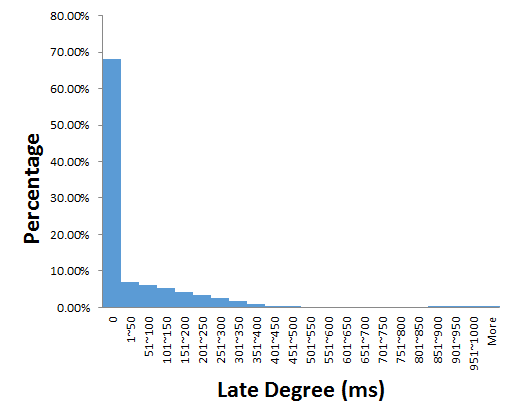
\includegraphics[width=2.5in]{late_degree_distribution-16min_A}
		\caption{Soccer-16min, Stream A}
		\hspace{5pt}
		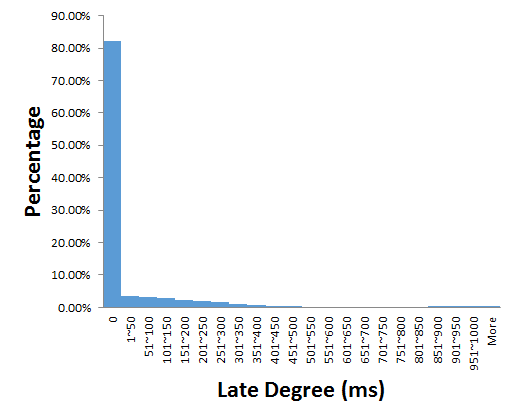
\includegraphics[width=2.5in]{late_degree_distribution-23min_A}
		\caption{Soccer-23min, Stream A}	
	\end{subfigure}
	\quad
	\begin{subfigure}[t]{2.4in}
		\centering
		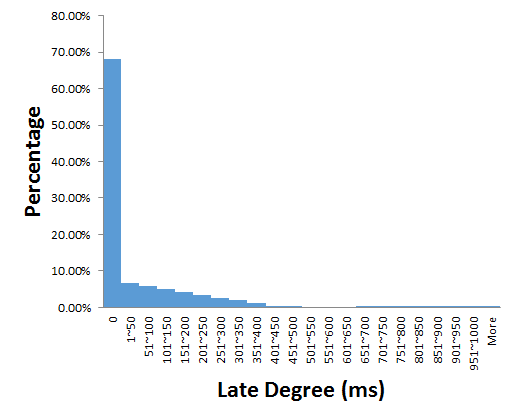
\includegraphics[width=2.5in]{late_degree_distribution-16min_B}
		\caption{Soccer-16min, Stream B}
		\hspace{5pt}
		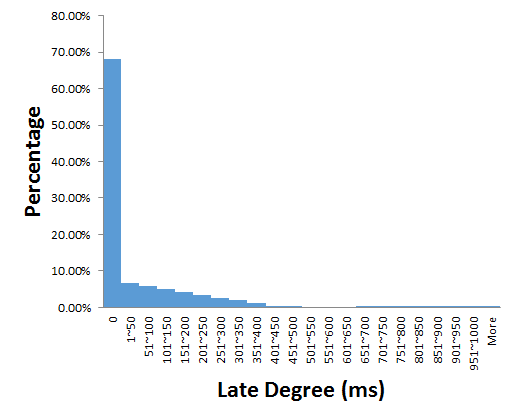
\includegraphics[width=2.5in]{late_degree_distribution-23min_B}
		\caption{Soccer-23min, Stream B}
	\end{subfigure}
	\caption{Overall late degree distribution of each stream used in the evaluation}\label{fig:dataset-late-degree-distribution}
\end{figure}

In order to demonstrate the inter-stream disorder of the two datasets, we draw the out-of-sync spectrums for them in Figure \ref{fig:out-of-sync-spectrum}. The x-axis is the number of tuple in the whole dataset, and the y-axis shows the difference between $clk_A$ and $clk_B$ at the time each tuple comes. As we can see, neither of the two streams stream is always leading or lagging, and the out-of-order degree vibrates within $\pm$50ms at most of the time.\\

\begin{figure}[h]
	\centering
	\begin{subfigure}[t]{5in}
		\centering
		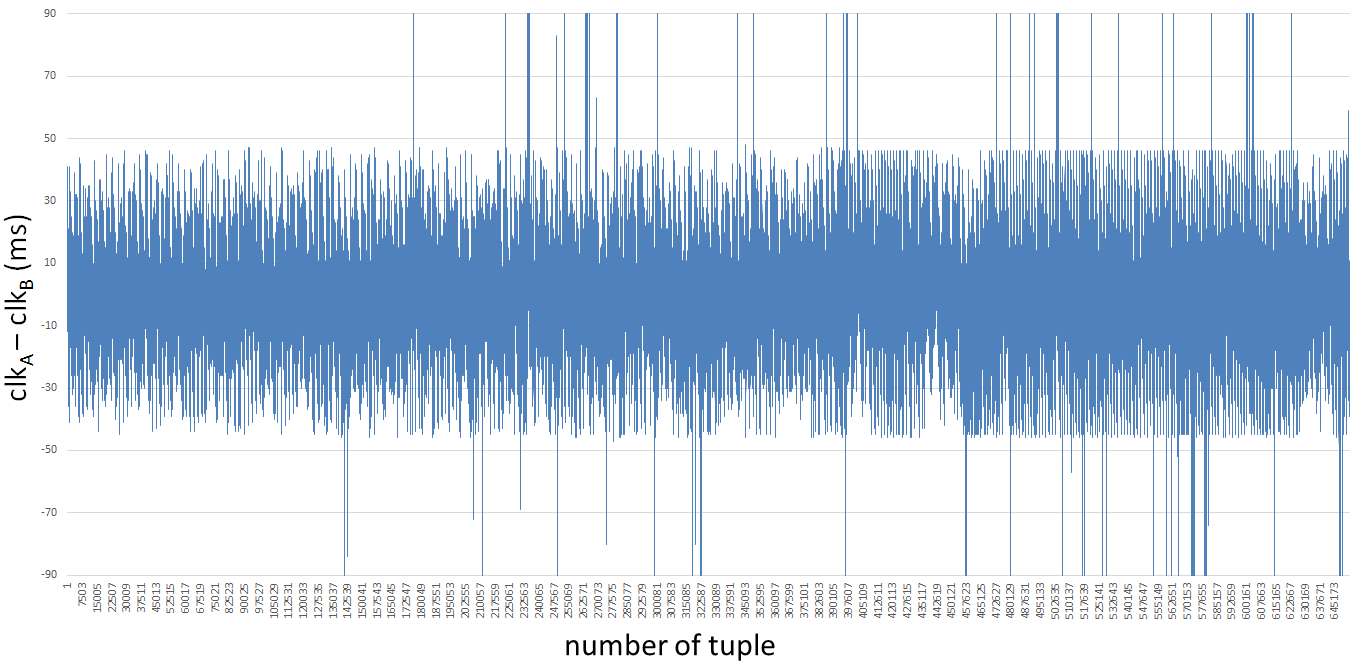
\includegraphics[width=5in]{spectrum-16min}
		\caption{Soccer-16min}
		\hspace{5pt}
		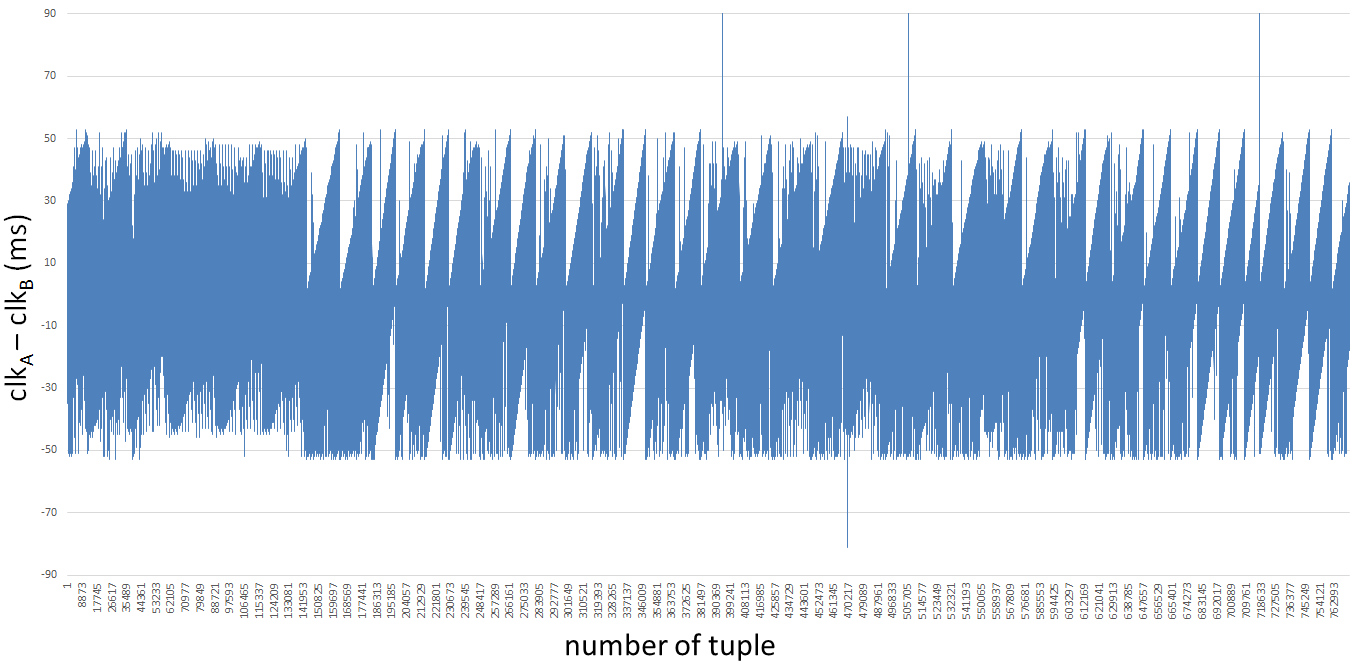
\includegraphics[width=5in]{spectrum-23min}
		\caption{Soccer-23min}	
	\end{subfigure}
	\caption{Out-of-sync spectrum of each dataset used in the evaluation}\label{fig:out-of-sync-spectrum}
\end{figure}

\subsection{Comparative Algorithm and Baselines}

In order to evaluate the performance of our approach, we choose the Proportional-Derivative (PD) Controller \cite{astrom1995pid} as a second slack size adaptation algorithm, which is used in \cite{Lisa}. The PD controller calculates an $error$ value as the difference between the result quality monitored by the quality tracker and the user-specified $quality\_expectation$. Then it attempts to minimize the $error$ by adjusting the \textit{K}-Slack size. The parameters $K_p$ and $K_d$ are tuned manually, based on the Ziegler-Nichols method \cite{ziegler1942optimum}.\\

In addition, we use three baselines.

\begin{itemize}
\item \texttt{Baseline1}: no \textit{K}-Slacks are applied;
\item \texttt{Baseline2}: \textit{SyncBuffer} and \textit{K}-Slacks with minimum size that can guarantee 100\% result quality are applied;
\item \texttt{Baseline3}: no \textit{SyncBuffer} nor \textit{K}-Slacks are applied.
\end{itemize}

\section{Experiment Results}
\label{sec:experiment results}

In this section, we first use common parameter settings and compare the performance of our disorder handling approach with the PD controller and baselines in Section \ref{subsec:basic-experiment}. Then we variate the parameters to see their influences to our approach in Section \ref{subsec:influence-parameters}. At last, we measure the computational overhead caused by our disorder handling components in Section \ref{subsec:computational-overhead}.

\subsection{Basic Experiment}
\label{subsec:basic-experiment}

We use the following query to evaluate the algorithms. Window A has a size of two second, and Window B has a size of three seconds. The window slide unit $U$=10ms.

\begin{verbatim}
SELECT 
  MAX(A.Timestamp, B.Timestamp) as Timestamp, A.Value, B.Value
FROM StreamA as A KEEP 2 SECOND, StreamB as B KEEP 3 SECOND
SLIDE 10 MILLISECOND
\end{verbatim}

The parameter settings are listed in Table \ref{table:parameter-setup}.\\

\begin{table}[h]
\begin{center}
\begin{tabular}{|c|c|}
\hline
Parameter                    & Value                  \\ \hline
$optimize\_overall\_quality$ & true/false             \\ \hline
$quality\_track\_duration$   & 1000ms                 \\ \hline
$k\_granularity$             & 10ms                   \\ \hline
$decay\_factor$         	 & 0.8                    \\ \hline
$quality\_expectation$       & 80\%, 90\%, 95\%, 98\% \\ \hline
\end{tabular}
\caption{Standard parameter setup\label{table:parameter-setup}}
\end{center}
\end{table}

In order to compare the performance of the algorithms, we measure two essential metrics for each query execution:\\

\begin{description}
\item[I. Quality Compliance Rate (QCR)]\hspace*{\fill} \\

For each quality track duration, we test if the result quality within this duration meets the user-specified $quality\_expectation$. The \emph{quality compliance rate} is calculated as the number of quality track durations during which the actual result quality does not violate the user-specified $quality\_expectation$, divided by the total number of quality track durations during the entire query execution.\\

\item[II. Average Buffer Size (ABS)]\hspace*{\fill} \\

The average buffer size within each quality track duration, including the size of \textit{K}-Slacks and the size of \textit{SyncBuffer}. It can be seen as the average result delay caused by the disorder handling.\\
\end{description}

We then calculate and compare QCR/ABS value. For the same dataset with coordinate setting, if Algorithm A produces higher QCR/ABS than Algorithm B, we consider A outperforms B, because it can trade one unit of delay time for higher result quality.\\

\clearpage
\subsubsection{Buffer Size Adaptation based on Quality within Individual Quality Track Duration}
\label{subsec:optimize-quality-for-each-duration}

We first set $optimize\_overall\_quality$ to false, namely, to perform buffer size adaptation based on the result quality within each individual quality track duration. We evaluate the performance of each algorithm and baseline over both \texttt{Soccer-16min} and \texttt{Soccer-23min}. The results are shown on the next pages.\\

\clearpage

The average buffer size (ABS) used in each execution is listed in Figure \ref{fig:average-buffer-size}. Because \texttt{Baseline2} uses significantly large buffer, its buffer size is not shown in the bar chart. In general, the better the result quality that the user expects, the larger the buffer size that quality-driven buffer size adaptation approaches (our approach and the PD controller) use. Overall, our approach uses approximately 10\% to 24\% more buffer size compared with the PD controller, and the better the quality that the user expects, the larger the difference is.\\

\begin{figure}[!hb]
	\centering
	\begin{subfigure}[t]{5in}
		\centering
		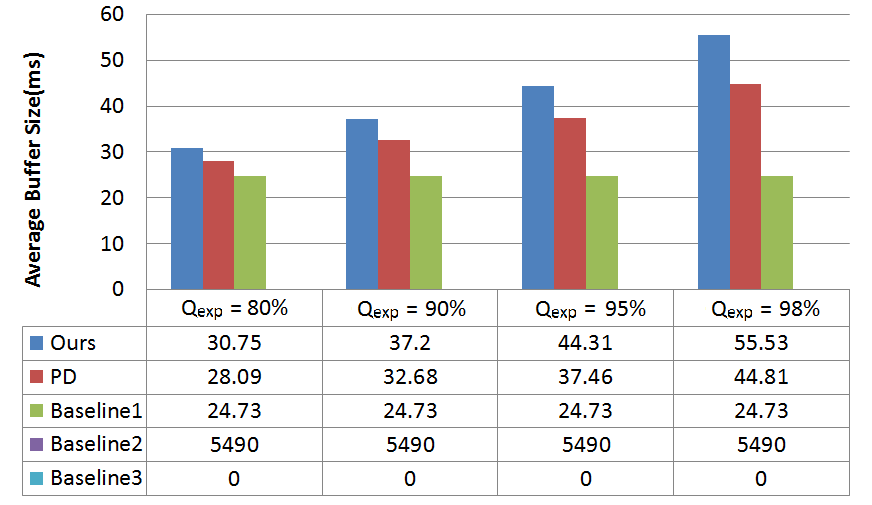
\includegraphics[width=5in]{average-buffer-size-16min}
		\caption{Soccer-16min}
		\hspace{5pt}
		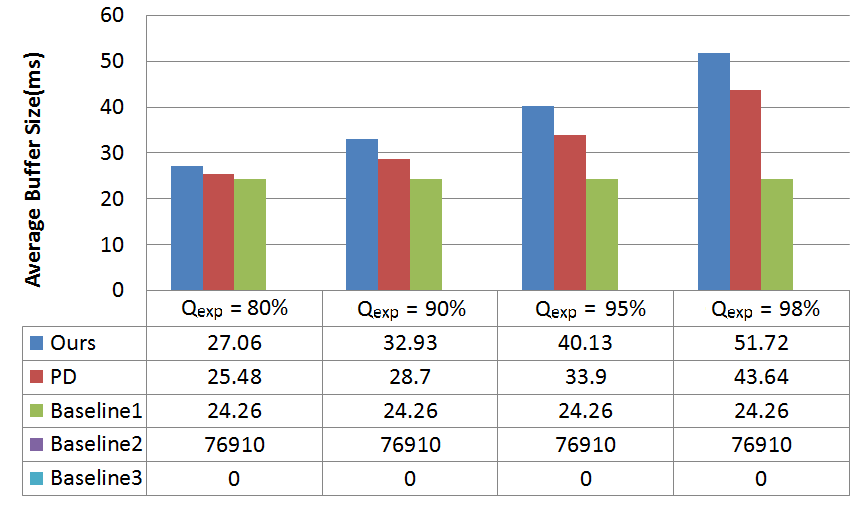
\includegraphics[width=5in]{average-buffer-size-23min}
		\caption{Soccer-23min}	
	\end{subfigure}
	\caption{Average buffer size (ABS) ($optimize\_overall\_quality$ = false)}
	\label{fig:average-buffer-size}
\end{figure}

However, our approach has better quality compliance rate (QCR) performance than the PD controller, as shown in Figure \ref{fig:quality-compliance-rate}. In general, though both quality-driven approaches exhibit decrease as the $quality\_expectation$ increases, our approach has higher QCR than the PD controller in every execution. Moreover, the PD controller has more serious decrease: from 79.21\% to 64.40\% for \texttt{Soccer-16min}, and from 88.99\% to 64.32\% for \texttt{Soccer-23min}; while the decrease of our approach is smaller: from 93.20\% to 90.06\% for \texttt{Soccer-16min}, and from 94.35\% to 87.18\% for \texttt{Soccer-23min}.\\

\begin{figure}[H]
	\centering
	\begin{subfigure}[t]{5in}
		\centering
		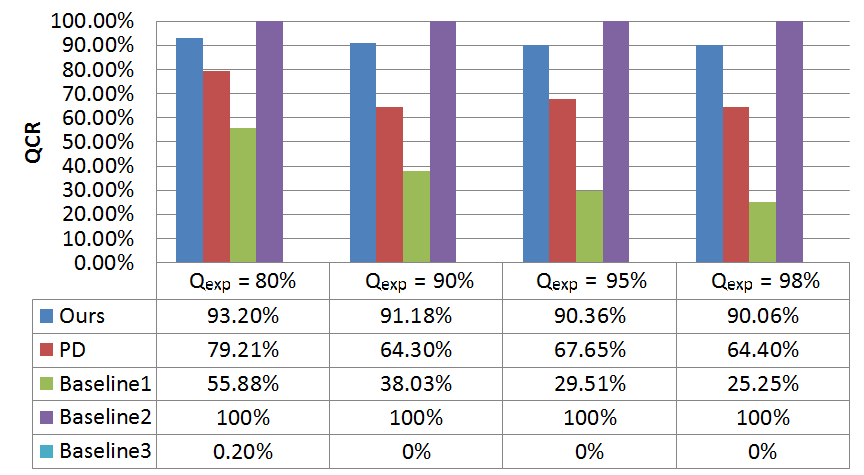
\includegraphics[width=5in]{QCR-16min}
		\caption{Soccer-16min}
		\hspace{5pt}
		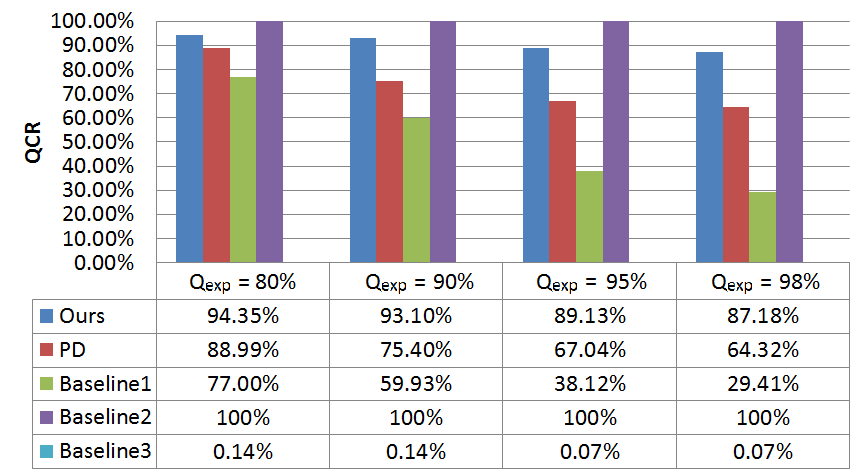
\includegraphics[width=5in]{QCR-23min}
		\caption{Soccer-23min}	
	\end{subfigure}
	\caption{Quality compliance rate (QCR) ($optimize\_overall\_quality$ = false)}
	\label{fig:quality-compliance-rate}
\end{figure}

We further calculate the QCR/ABS value for each execution in Figure \ref{fig:qcr/abs}. From this figure we can see that, the QCR/ABS value decreases as the \emph{quality\_expectation} increases, which indicates that we need to trade more buffer size for higher result quality. Overall, our approach has better QCR/ABS performance than the PD controller, for both \texttt{Soccer-16min} and \texttt{Soccer-23min}, with the only exception when $quality\_expectation=80\%$ for \texttt{Soccer-23min}, where both of them has QCR/ABS=3.49.

\begin{figure}[H]
	\centering
	\begin{subfigure}[t]{5in}
		\centering
		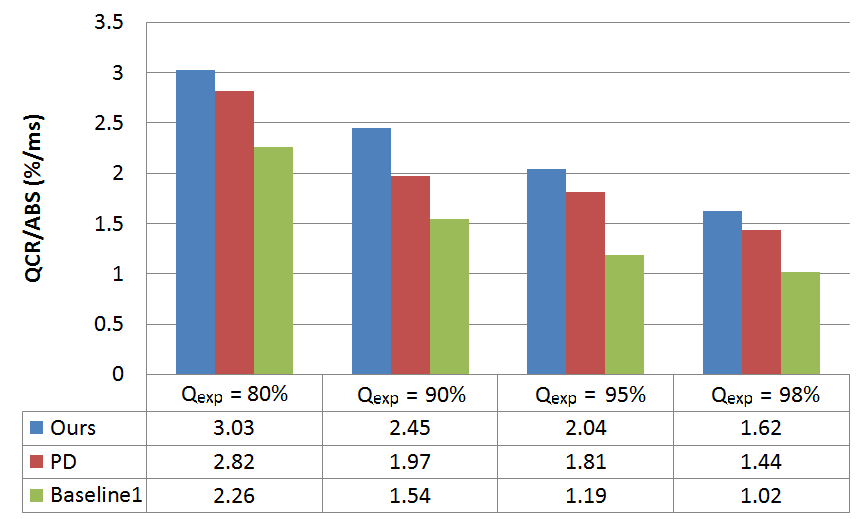
\includegraphics[width=5in]{QCR_ABS-16min}
		\caption{Soccer-16min}
		\hspace{5pt}
		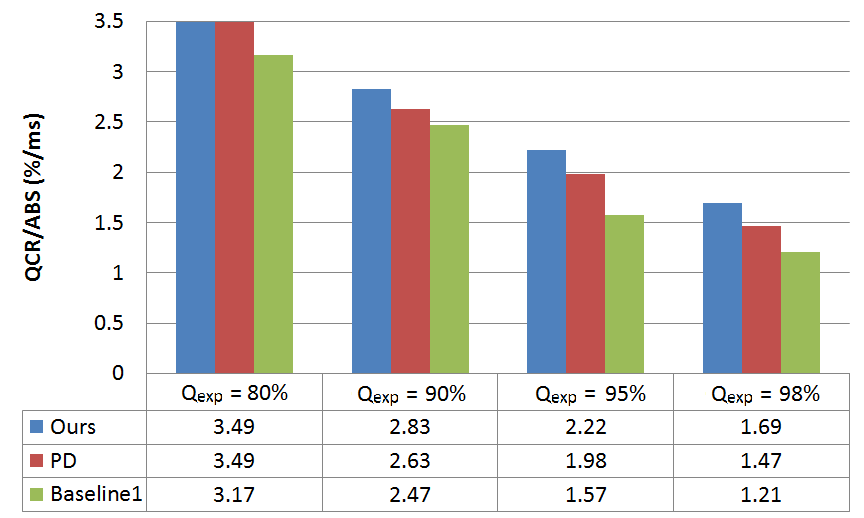
\includegraphics[width=5in]{QCR_ABS-23min}
		\caption{Soccer-23min}	
	\end{subfigure}
	\caption{QCR/ABS ($optimize\_overall\_quality$ = false)}
	\label{fig:qcr/abs}
\end{figure}



\subsubsection{Buffer Size Adaptation based on Overall Quality}
\label{subsec:optimize-overall-quality}

We define the overall quality as the result quality from the beginning of the execution to the current time, i.e., the total $Nr_{produced}$ divided by the total $Nr_{original}$ from the beginning of the execution. In case a user wants the overall quality to meet his requirement, he should set the parameter $optimize\_overall\_quality$ to true. In this subsection, we evaluate the performance of each algorithm and baseline under this circumstance. The results are shown on the next pages.\\

\clearpage

As shown in Figure \ref{fig:average-buffer-size-overallquality}, similar to the case when we perform buffer size adaptation based on the result quality within individual quality track duration, the higher the result quality that the user requires, the bigger the buffer size that we need. However, when we perform buffer size adaptation based on overall quality, our approach uses less buffer size on average than the PD controller in most cases, which is opposite to the situation when based on the result quality within individual quality track duration.\\

\begin{figure}[H]
	\centering
	\begin{subfigure}[t]{5in}
		\centering
		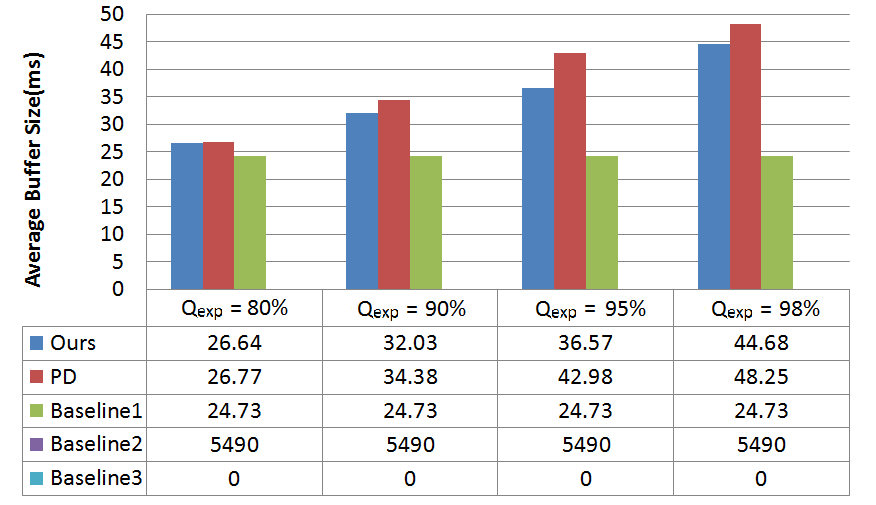
\includegraphics[width=5in]{average-buffer-size-16min-overallquality}
		\caption{Soccer-16min}
		\hspace{5pt}
		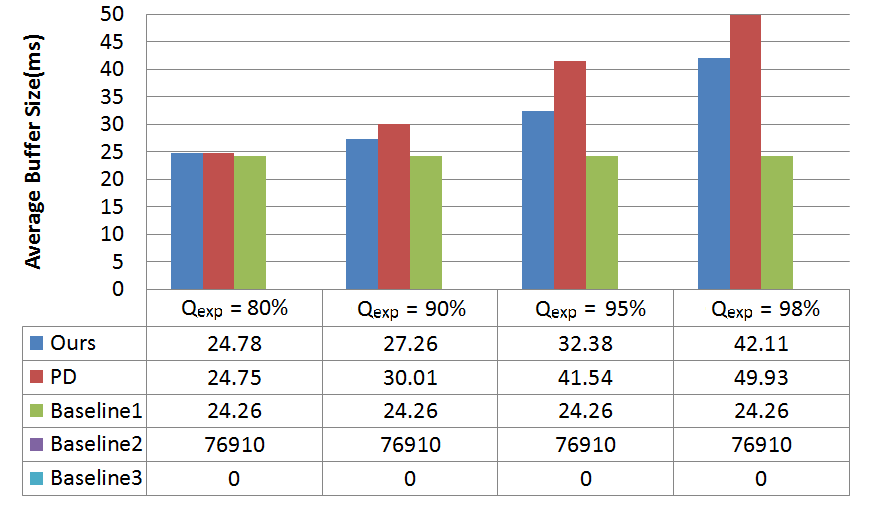
\includegraphics[width=5in]{average-buffer-size-23min-overallquality}
		\caption{Soccer-23min}	
	\end{subfigure}
	\caption{Average buffer size (ABS) ($optimize\_overall\_quality$ = true)}
	\label{fig:average-buffer-size-overallquality}
\end{figure}

From Figure \ref {fig:quality-compliance-rate-overallquality} we can see that, QCR decreases as the $quality\_expectation$ increases in nearly all cases, except for the PD controller when \emph{quality\_expectation} is set to 98\% in both datasets. \texttt{Baseline1} has the most significant decrease. Its overall quality seldom meets the user's expectation, when the user has high quality requirement. However, QCR of our approach does not demonstrate significant decrease as the $quality\_expectation$ increases, compared to the PD controller. With the worst case when $quality\_expectation=98\%$ in \texttt{Soccer-23min}, our approach can still get a QCR of 93.17\%. The final result quality of \texttt{Soccer-23min} when $quality\_expectation=98\%$ with the PD controller is 97.88\%, not fulfilling user's demand.

\begin{figure}[H]
	\centering
	\begin{subfigure}[t]{5in}
		\centering
		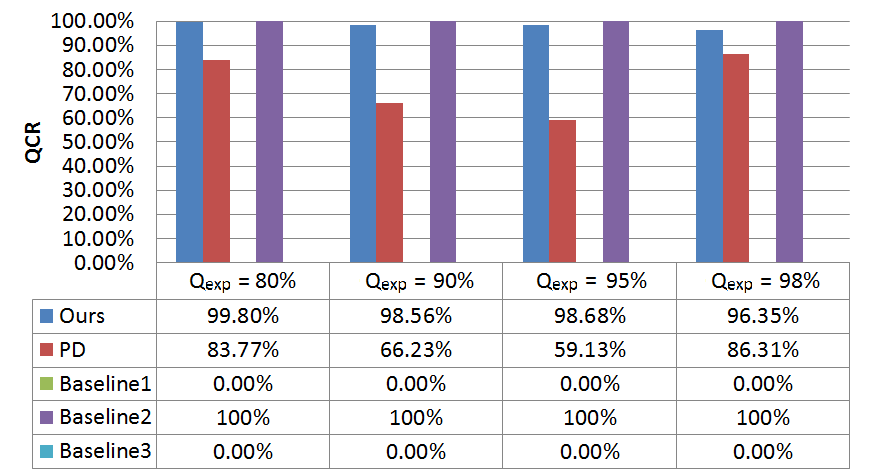
\includegraphics[width=5in]{QCR-16min-overallquality}
		\caption{Soccer-16min}
		\hspace{5pt}
		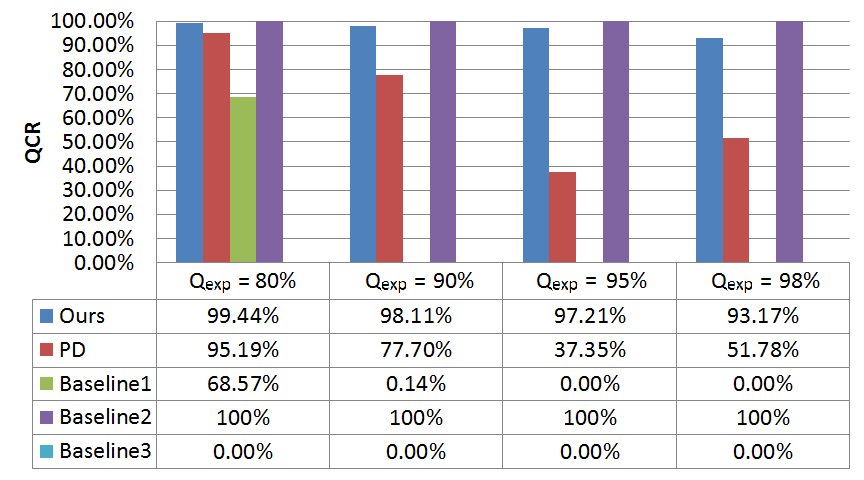
\includegraphics[width=5in]{QCR-23min-overallquality}
		\caption{Soccer-23min}	
	\end{subfigure}
	\caption{Quality compliance rate (QCR) ($optimize\_overall\_quality$ = true)}
	\label{fig:quality-compliance-rate-overallquality}
\end{figure}

Since in most cases our approach has smaller ABS and higher QCR than the PD controller, it is obvious that our approach would have higher QCR/ABS compared to the PD controller, as corroborated by the results in Figure \ref{fig:qcr/abs-overallquality}. Overall, when we perform buffer size adaptation based on overall quality, our approach also has higher QCR/ABS than the PD controller, for both \texttt{Soccer-16min} and \texttt{Soccer-23min}.\\

\begin{figure}[H]
	\centering
	\begin{subfigure}[t]{5in}
		\centering
		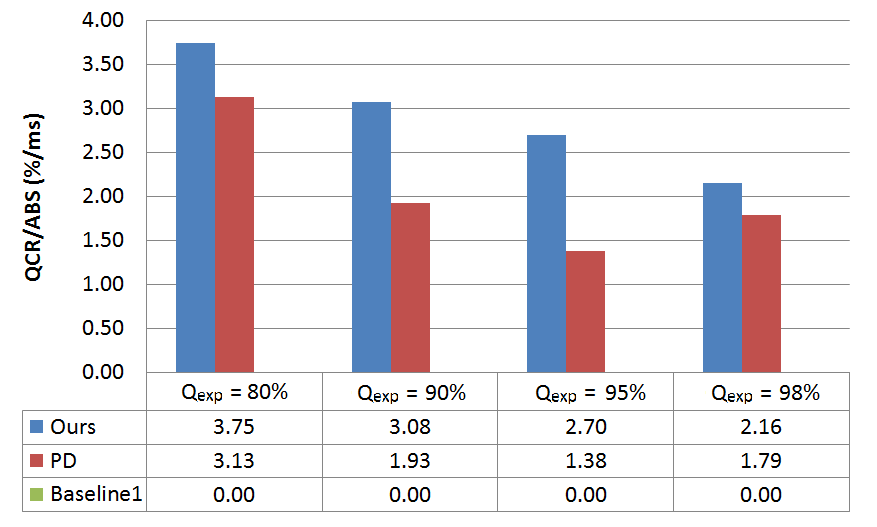
\includegraphics[width=5in]{QCR_ABS-16min-overallquality}
		\caption{Soccer-16min}
		\hspace{5pt}
		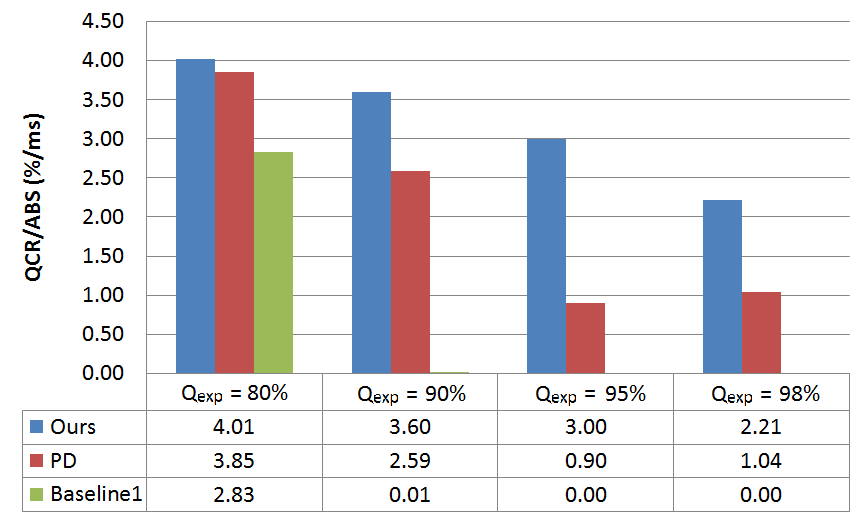
\includegraphics[width=5in]{QCR_ABS-23min-overallquality}
		\caption{Soccer-23min}	
	\end{subfigure}
	\caption{QCR/ABS ($optimize\_overall\_quality$ = true)}
	\label{fig:qcr/abs-overallquality}
\end{figure}



\subsubsection{Comparison between the Two Quality Targets}

In order to compare the two result quality targets (result quality within individual quality track duration and the overall quality) based on which we perform buffer size adaptation, we cross compare the experiment results in Section \ref{subsec:optimize-quality-for-each-duration} and Section \ref{subsec:optimize-overall-quality}.\\

Cross comparing Figure \ref{fig:average-buffer-size} and Figure \ref{fig:average-buffer-size-overallquality} we can see that, for both datasets and all $quality\_expectation$ settings, our approach consumes less average buffer size when we perform buffer size adaptation based on overall quality, than based on result quality within individual quality track duration. The PD controller has the opposite situation, except for the case where $quality\_expectation$ is set to 80\%, the PD controller also consumes less average buffer size when performing buffer size adaptation based on overall quality, than based on result quality within individual quality track duration.\\

Cross comparing Figure \ref{fig:quality-compliance-rate} and Figure \ref{fig:quality-compliance-rate-overallquality} we can see that, for both datasets and all $quality\_expectation$ settings, our approach achieves better QCR when performing buffer size adaptation based on overall quality, than based on result quality within individual quality track duration. We do not see a clear pattern for the PD controller.\\

Figure \ref{fig:quality-plot} presents the result quality change during the whole executions using common settings, one performing buffer size adaptation based on result quality within individual quality track duration (Figure \ref{fig:quality-plot-a}), and the other based on overall quality (Figure \ref{fig:quality-plot-b}). The curves of both our approach and the PD controller in Figure \ref{fig:quality-plot-b} are much smoother than the ones in Figure \ref{fig:quality-plot-a}. The reason is that, the result quality of one quality track duration has little impact on the result quality of another; while as the total $Nr_{produced}$ and $Nr_{original}$ grow bigger, the overall quality calculated in one quality track duration has higher and higher impact on the overall quality calculated in the next quality track duration.\\

This also explains why the the PD controller has bad performance when performing buffer size adaptation based on overall quality. According to the algorithm of the PD controller, it only increases $K$ when the overall quality is smaller than $quality\_expectation$. However, when performing buffer size adaptation based on overall quality, in the late period of the execution, when the the total $Nr_{produced}$ and $Nr_{original}$ is very large, even an overall quality which is slightly smaller than $quality\_expectation$ has significant impact on the later values of overall quality. However, according to the algorithm of the PD controller, it will only increase $K$ a little bit, which cannot stop the further decrease of the overall quality. This case is shown in Figure \ref{fig:quality-plot-b}, the overall quality of the PD controller continues to decrease after it gets smaller than $quality\_expectation$. On the contrary, our approach adjusts $K$ based on estimation of future result quality. Therefore, it could increase $K$ even if the overall quality is not smaller than $quality\_expectation$.\\

\begin{figure}[H]
	\centering
	\begin{subfigure}[t]{5in}
		\centering
		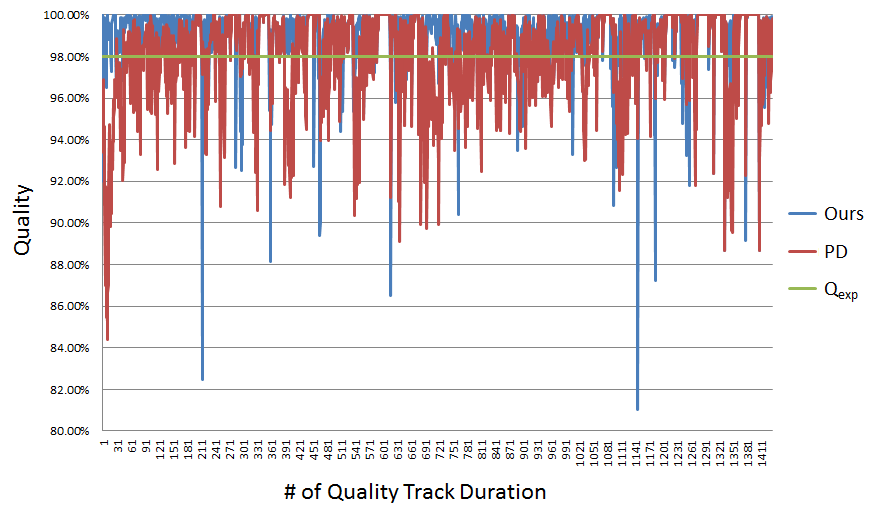
\includegraphics[width=5in]{quality-plot}
		\caption{Optimizing quality for each quality track duration}
		\label{fig:quality-plot-a}
		\hspace{5pt}
		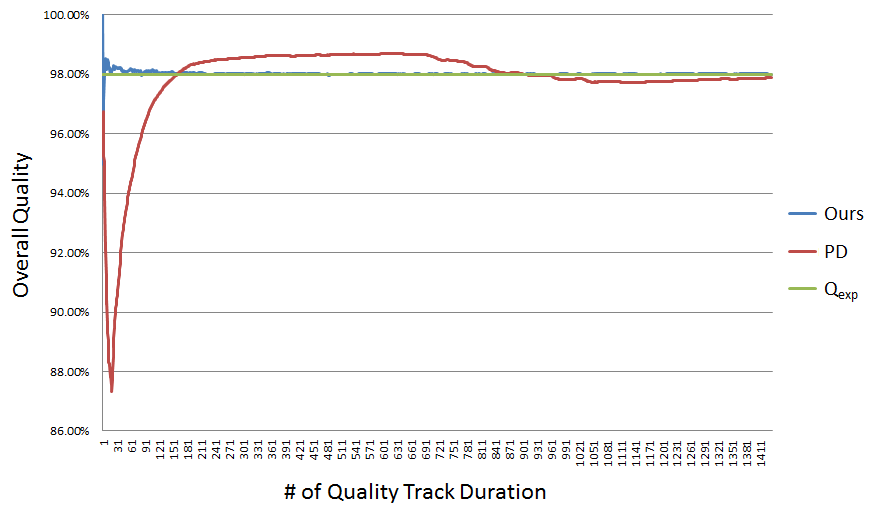
\includegraphics[width=5in]{quality-plot-overallquality}
		\caption{Optimizing overall quality}	
		\label{fig:quality-plot-b}
	\end{subfigure}
	\caption{Quality plot (Soccer-23min, $quality\_expectation$=98\%)}
	\label{fig:quality-plot}
\end{figure}

Cross comparing Figure \ref{fig:qcr/abs} and Figure \ref{fig:qcr/abs-overallquality}, we can see that, our approach gets higher QCR/ABS in most cases. This indicates that our approach is more suitable than the PD controller for quality-driven buffer size adaptation, since it can trade oneunit of delay time for higher result quality. Besides, the QCR/ABS of our approach is higher in Figure \ref{fig:qcr/abs-overallquality} than in Figure \ref{fig:qcr/abs}, which indicates that it is easier for our approach to provide better result quality with smaller buffer size (i.e., smaller result delay), when it performs buffer size adaptation based on overall quality, than based on result quality within individual quality track duration.\\

\clearpage

\subsection{Influence of Parameters}
\label{subsec:influence-parameters}

In this subsection, we evaluate the influence of the three parameters: \emph{quality\_track\_duration}, $k\_granularity$ and $decay\_factor$ to our approach. For each of them, we fix the other parameters and test the QCR/ABS performance under varying settings of this parameter, with both datasets and the four $quality\_expectation$ settings: 80\%, 90\%, 95\% and 98\%. We take the default setting of quality target, i.e., to perform buffer size adaptation based on result quality within individual quality track duration.\\

\subsubsection{Influence of \textit{quality\_track\_duration}}
\label{subsec:influence-quality-track-duration}

As we have already explained in Section \ref{subsec:estimation-of-quality}, the setting of the time interval $T$ (i.e., parameter $quality\_track\_duration$) for which we estimate the result quality is important to our approach. In order to evaluate its influence, we fix other parameters and vary $quality\_track\_duration$ from 500ms to 2000ms, and compare their QCR/ABS performance.\\

From Figure \ref{fig:influence-quality-track-duration} we can see that, for both \texttt{Soccer-16min} and \texttt{Soccer-23min}, the QCR/ABS performance of our approach under three different settings of $quality\_track\_duration$ are roughly equivalent (with a deviation of $\pm 3\%$ compared to the standard setting 1000ms), when $quality\_expectation$ is set to 80\%, 90\% and 95\%. When we have $quality\_expectation$=98\%, for \texttt{Soccer-16min}, the QCR/ABS performance under the setting \emph{quality\_track\_duration} = 500ms is significantly decreased (-22.8\% compared to the standard setting); while the QCR/ABS performance under the setting \emph{quality\_track\_duration} = 2000ms is seen improved by 5.6\% compared to the standard setting. The reason could be that, \texttt{Soccer-16min} has fewer result tuples per second. In this case, according to the discussions in Section \ref{subsec:estimation-of-quality}, when we have shorter $quality\_track\_duration$, the result quality estimation is less accurate, vice versa.\\

\clearpage

\begin{figure}[H]
	\centering
	\begin{subfigure}[t]{5in}
		\centering
		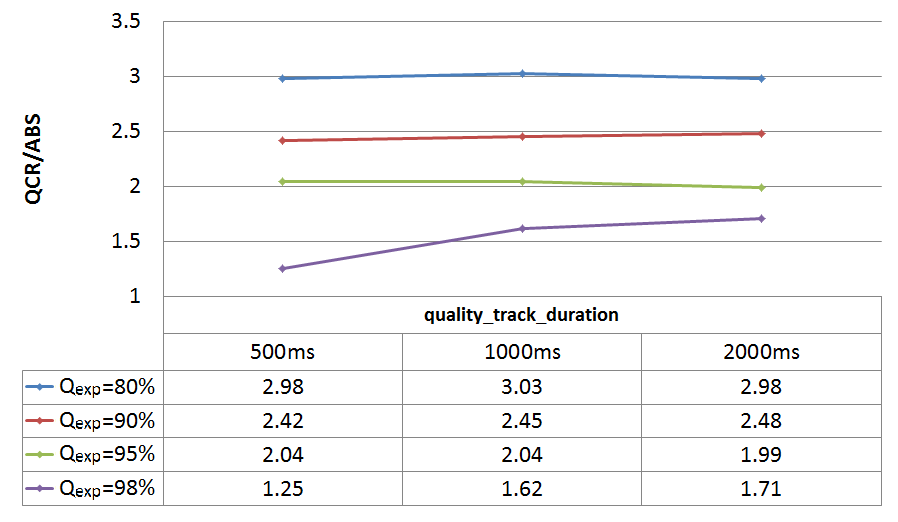
\includegraphics[width=5in]{influence-quality-track-duration-16min}
		\caption{Soccer-16min}
		\hspace{5pt}
		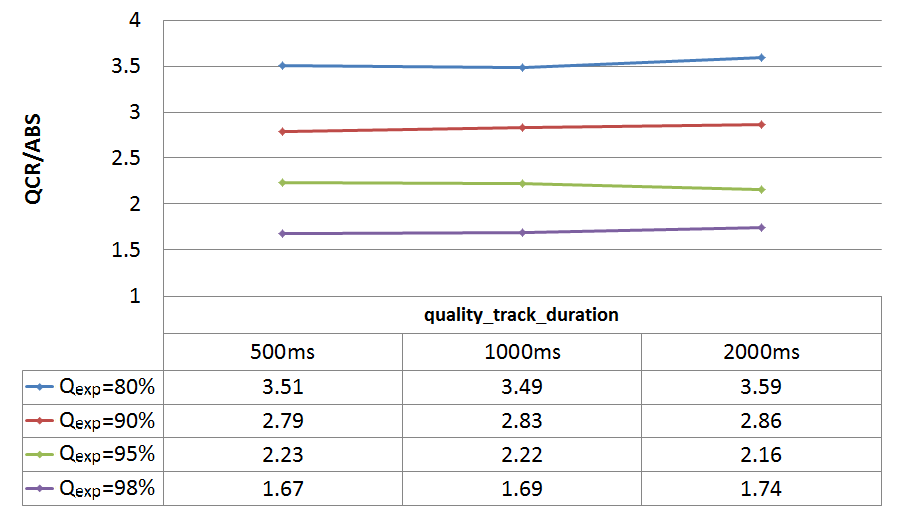
\includegraphics[width=5in]{influence-quality-track-duration-23min}
		\caption{Soccer-23min}	
	\end{subfigure}
	\caption{Influence of $quality\_track\_duration$ \protect\\ ($k\_granularity$ = 10ms, $decay\_factor$ = 0.8)}
	\label{fig:influence-quality-track-duration}
\end{figure}

\clearpage

\subsubsection{Influence of \textit{k\_granularity}}
\label{subsec:influence-k-granularity}

The parameter $k\_granularity$ defines the granularity we adjust the size of \textit{K}-Slacks. We fix other parameters and vary $k\_granularity$, in order to find its influence on the performance of our approach. Figure \ref{fig:influence-k-granularity} shows the QCR/ABS performance when  $k\_granularity$ is set to 2.5ms, 5ms and 10ms.\\

\begin{figure}[H]
	\centering
	\begin{subfigure}[t]{5in}
		\centering
		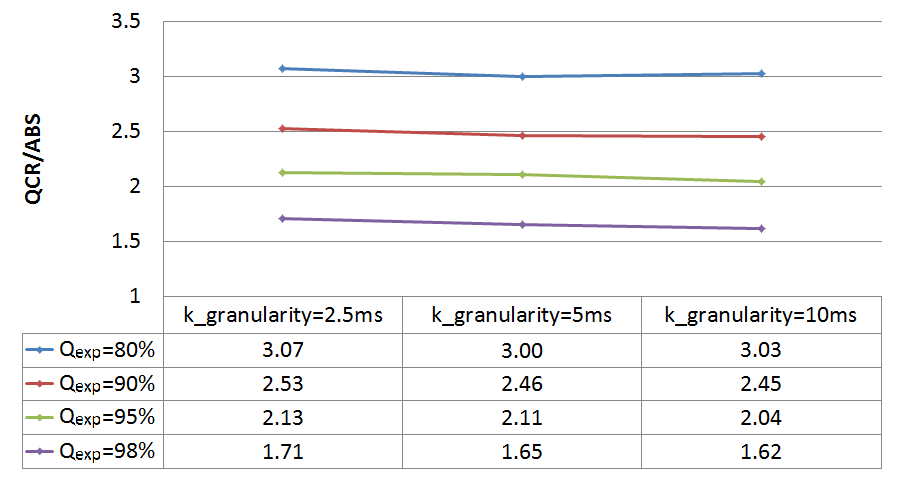
\includegraphics[width=5in]{influence-k-granularity-16min}
		\caption{Soccer-16min}
		\hspace{5pt}
		\includegraphics[width=5in]{influence-k-granularity-23min}
		\caption{Soccer-23min}	
	\end{subfigure}
	\caption{Influence of $k\_granularity$ \protect\\ ($quality\_track\_duration$ = 1000ms, $decay\_factor$ = 0.8)}
	\label{fig:influence-k-granularity}
\end{figure}

As shown in this figure, our approach has better performance with smaller $k\_granularity$ settings than with larger $k\_granularity$ settings in most cases. This can be explained by how we determines the buffer size. According to Algorithm \ref{algo:slack-size-adaptation}, we start the incremental search for suitable $K$ values from value zero, until the estimated quality is not smaller than $quality\_expectation$. Therefore, a smaller $k\_granularity$ setting will have a chance to result in smaller $K$ values, hence smaller buffer size. However, due to estimation errors, this smaller buffer size can sometimes result in a result quality lower than $quality\_expectation$. This explains the counterexample in \texttt{Soccer-16min}, when $quality\_expectation$ is 80\%; the QCR/ABS of the setting $k\_granularity$ = 5ms slightly worse than the QCR/ABS of the setting $k\_granularity$=10ms.\\

\clearpage

\subsubsection{Influence of \textit{decay\_factor}}
\label{subsec:influence-elimination-rate}

The parameter $decay\_factor$ controls how fast the system eliminates the influence of old late records, as explained in Section \ref{subsec:parameters} (the smaller the faster). In order to analyze the influence of $decay\_factor$ to our approach, we fix other parameters and vary $decay\_factor$. Figure \ref{fig:influence-elimination-rate} shows the QCR/ABS performance when $decay\_factor$ is set to 0.7, 0.8 and 0.9.\\

\begin{figure}[H]
	\centering
	\begin{subfigure}[t]{5in}
		\centering
		\includegraphics[width=5in]{influence-elimination-rate-16min}
		\caption{Soccer-16min}
		\hspace{5pt}
		\includegraphics[width=5in]{influence-elimination-rate-23min}
		\caption{Soccer-23min}	
	\end{subfigure}
	\caption{Influence of $decay\_factor$ \protect\\ ($quality\_track\_duration$ = 1000ms, $k\_granularity$ = 10ms)}
	\label{fig:influence-elimination-rate}
\end{figure}

From the figure we can see that, when $quality\_expectation$ is set to 80\%, 90\% and 95\%, there is little influence of the $decay\_factor$ setting (with a deviation of $\pm 2\%$ compared to the standard setting 0.8). Only when we set $quality\_expectation$ to 98\%, the setting $decay\_factor=0.7$ has significant decrease of performance (-5.6\% for \texttt{Soccerr-16min}, -11.8\% for \texttt{Soccerr-23min}, compared to the standard setting). This indicates that, it is not always better to eliminate the influence of old late records fast, because sometimes they are still valuable in revealing the pattern of tuples. Besides, it is also not optimal to do very slow decay, since we always want the newest records to have the biggest influence. Overall, our approach has the best performance when $decay\_factor$ is set to 0.8 in our test.\\

\clearpage

\subsection{Computational Overhead}
\label{subsec:computational-overhead}
In order to evaluate the computational overhead of the three disorder handling components, the \textit{late degree monitor}, the \textit{slack size adapter} and the \textit{quality tracker}, as mentioned in Section \ref{subsec:disorder handling components}, we measure and compare the execution times accomplishing JOIN executions over the same dataset with and without them.\\

Technically, we set a flag to enable and disable the three components in the code and use the same sorted data stream as input for these two different executions. The reason why the original unsorted data stream is not used is that, if we disable the three components, the inter-stream disorder will not be handled the same way as we enable them. This will lead to different join results because the operands of the join operator will be different. More specifically, when we disable the three components, more input tuples will be discarded, and, as a consequence, fewer join results will be produced, than when we enable the three components. Since join operations also take time, different join operations make it difficult to evaluate the execution time difference caused by the three disorder handling components. Using sorted data stream will totally avoid this problem, because the join operands will keep the same between the entire execution with disorder handling components, and the entire execution without them. In our experiment we use sorted \texttt{Soccer-23min} as input. We measure the total execution time five times for each condition and calculate the average total execution time. The results are listed in Table \ref{table:overhead-comparison}.\\

\begin{table}[h]
\begin{center}
\begin{tabular}{|c|c|c|}
\hline
No. experiment     & Enable components & Disable components \\ \hline
1                  & 1,375.440         & 1,364.174          \\ \hline
2                  & 1,366.799         & 1,386.612          \\ \hline
3                  & 1,379.475         & 1,346.368          \\ \hline
4                  & 1,346.852         & 1,367.247          \\ \hline
5                  & 1,377.083         & 1,382.139          \\ \hline
Average            & 1,369.130         & 1,369.308          \\ \hline
Standard error     & 13.340            & 15.976             \\ \hline
\end{tabular}
\caption{Execution time comparison (unit:sec)\label{table:overhead-comparison}}
\end{center}
\end{table}

The average execution time shows that the computational overhead caused by the three disorder handling components is negligible.\\

\cleardoublepage

\chapter{Conclusion}

In this thesis, we have focused on quality-driven sliding-window JOIN over data streams. Based on existing works, we have proposed our own a probabilistic model, aiming to reveal the relationship between buffer size and result quality. With estimation of future result quality based on observed late arrival pattern of the incoming data, our model can minimize the result latency while fulfilling users' requirement on result quality. We have implemented our proposal in SAP Sybase ESP system.\\

In the evaluation part, we have validated our quality-driven slack size adaptation approach using real world data. Experimental results have shown that, compared to the existing PD controller algorithm, our approach is more suitable for quality-driven slack size adaptation, when performing sliding-window JOIN over data streams. The influence of parameters to our approach has also been evaluated.\\

Although the implemented solution has shown its effectiveness, there exists a wide range of aspects for future works and improvements. First, we have only implemented sliding-window JOIN over two data streams. In principle, our approach can be extended and used in a variety of operators (e.g., UNION, INTERSECT) over multiple data streams. Second, in the evaluation part, we have only tested the case when the join selectivity $\rho=100\%$, while the case when $\rho$ is not always 100\% remains unstudied.



\cleardoublepage

\renewcommand{\nomname}{List of Notations}
\label{nomenclature}
\printnomenclature

\listoffigures

\listoftables

\cleardoublepage
\bibliography{ref}
\bibliographystyle{plain}

\cleardoublepage
 
\end{document}
